%%%%%%%%%%%%%%%%%%%%%%%%%%%%%%%%%%%%%%%%%%%%%%%%%%%%%%%%%%%%%%%%%%%%%%%%%%%%%%%%
% Main TeX file for PhD thesis
%%%%%%%%%%%%%%%%%%%%%%%%%%%%%%%%%%%%%%%%%%%%%%%%%%%%%%%%%%%%%%%%%%%%%%%%%%%%%%%%


%%%%%%%%%%%%%%%%%%%%%%%%%%%%%%%%%%%%%%%%%%%%%%%%%%%%%%%%%%%%%%%%%%%%%%%%%%%%%%%%
% Formatting and package includes
%%%%%%%%%%%%%%%%%%%%%%%%%%%%%%%%%%%%%%%%%%%%%%%%%%%%%%%%%%%%%%%%%%%%%%%%%%%%%%%%
\documentclass[12pt,a4paper,twoside]{book}
%--------------------------------------------------------------------------------
% Make figures stick to the top of the page, when there is no text.
% For example, on the last page of a chapter.
%--------------------------------------------------------------------------------
\makeatletter
\setlength{\@fptop}{0pt}
\makeatother
\PassOptionsToPackage{english}{babel}
%%%%%%%%%%%%%%%%%%%%%%%%%%%%%%%%%%%%%%%%%%%%%%%%%%%%%%%%%%%%%%%%%%%%%%%%%%%%%%%%
% Thesis formatting style
%%%%%%%%%%%%%%%%%%%%%%%%%%%%%%%%%%%%%%%%%%%%%%%%%%%%%%%%%%%%%%%%%%%%%%%%%%%%%%%%


%--------------------------------------------------------------------------------
% Packages
%--------------------------------------------------------------------------------
\usepackage{times}

\usepackage{color}				% Allow colored text
\usepackage{graphicx}			% Allow graphics

\usepackage{fancyhdr}			% Custom headers
\usepackage{enumerate}			% Custom enum
\usepackage{cite}				% otherwise citations are not set nicely

\usepackage{algorithm}
\usepackage{algorithmic}
\usepackage{subfigure}
\usepackage{amsmath}
\usepackage{amssymb}

\usepackage{tabularx}
\usepackage{array}
\usepackage{CV}


%--------------------------------------------------------------------------------
% Define colors
%--------------------------------------------------------------------------------
\definecolor{RED}{RGB}{255,0,0}
\definecolor{GREEN}{RGB}{0,255,0}
\definecolor{BLUE}{RGB}{0,0,255}
\definecolor{GRAY}{RGB}{128,128,128}
\definecolor{BLACK}{RGB}{0,0,0}


%--------------------------------------------------------------------------------
% Useful Commands
%--------------------------------------------------------------------------------
\newcommand{\RENATO}[1]{\textbf{\color{RED}{RENATO: #1}}}
\newcommand{\FATIH}[1]{\textbf{\color{GREEN}{FATIH: #1}}}

\newcommand{\itemtitle}[1]{\addtolength{\parskip}{3mm}{\noindent\bf {#1}} \addtolength{\parskip}{-3mm}}

% Define degree command
\newcommand{\degree}{\ensuremath{^\circ}}


%--------------------------------------------------------------------------------
% Book layout
%--------------------------------------------------------------------------------
\input{letterspacing.tex} % define the spacing between letters -> used for the word chapter
\usepackage[nottoc]{tocbibind} % used to include bibliography in the table of contents

% PDF bookmarks
% \usepackage[bookmarks=true,bookmarksnumbered=true]{hyperref}

\usepackage{xspace}

\hyphenation{Leap-frog}


% Manually set margins, so that the bigger space is on correct side
\setlength\oddsidemargin{0.7in}
\setlength\evensidemargin{0.14in}


%--------------------------------------------------------------------------------
% Headers and Footers
%--------------------------------------------------------------------------------
\pagestyle{fancy}
\fancyhf{}

\renewcommand{\chaptermark}[1]{%
\markboth{\MakeUppercase{\thechapter \space \ #1}}{}}

\renewcommand{\sectionmark}[1]{\markright{\thesection \space\ #1}}

\fancyhead[LE,RO]{\footnotesize\usefont{T1}{fvs}{n}{n}\selectfont\thepage}
\fancyhead[RE]{\footnotesize \usefont{T1}{fvs}{n}{n}\selectfont{\leftmark}}
\fancyhead[LO]{\footnotesize\usefont{T1}{fvs}{n}{n}\selectfont{\rightmark}}
\headsep 1cm % abstand header - text

% Chapters have to start on an odd page. So, if the chapter before ended on odd page, there is an empty page
% inbetween, which still gets header and footer that looks bad. We redefine how LaTeX adds the empty page.
\makeatletter
\def\cleardoublepage{\clearpage\if@twoside \ifodd\c@page\else
\hbox{}
\thispagestyle{empty}
\newpage
\if@twocolumn\hbox{}\newpage\fi\fi\fi}
\makeatother


%--------------------------------------------------------------------------------
% Section titles
%--------------------------------------------------------------------------------
\usepackage{sectsty}
\allsectionsfont{\large \usefont{T1}{fvs}{b}{n}\selectfont}
\subsectionfont{\normalsize \usefont{T1}{fvs}{b}{n}\selectfont}
\subsubsectionfont{\small \usefont{T1}{fvs}{b}{n}\selectfont}
\paragraphfont{\small \usefont{T1}{fvs}{b}{n}\selectfont}


%--------------------------------------------------------------------------------
% Chapter titles
%--------------------------------------------------------------------------------
\definecolor{NUMCOLOR}{rgb}{0.22,0.37,0.56}

\usepackage{multirow} % for tables with multiple rows

% The first makeatletter is to define the chapter layout in the real "Chapter" chapters
\makeatletter
\def\@makechapterhead#1{%
 % \vspace*{10\p@}%
  %\hrule

  \line(1,0){0}
  \newline
  {
  	 %\begin{tabular}{|@{}l|r@{}@{}|}
	 \begin{tabular}{@{}lr@{}@{}}
	 %\hline
	 \linethickness{ 4px }\color{NUMCOLOR}\line(1,0){245}
	& \multirow{2}{*}{\fontsize{100}{62}\usefont{OT1}{ptm}{m}{n}\selectfont \color{NUMCOLOR} \thechapter}\\ % ptm
	 & \\
	% \Huge \bfseries \usefont{OT1}{phv}{m}{n}\selectfont \scshape\@chapapp \hspace{8.25cm} & \\
	%\scshape \bfseries\Huge \@chapapp \hspace{8.25cm}
	\scshape \LARGE \usefont{T1}{fvs}{sc}{n}\selectfont \letterspace to 2.5\naturalwidth{CHAPTER} \hspace{3cm}
	& \\
	%\hline
	\end{tabular}

\vskip 100\p@
\raggedleft
    \interlinepenalty\@M
    \scshape \fontsize{24}{30} \usefont{T1}{fvs}{n}{n}\selectfont \scshape \MakeUppercase{#1}\par\nobreak
      \vskip 80\p@%60
  }
  }


% The second makeatletter is to define the chapter layout in the chapters like Abstract etc. (almost identical but without the word "chapter" and some ugly hacks which are necessary to align the titles)
\makeatletter
\def\@makeschapterhead#1{%
 % \vspace*{10\p@}%
  %\hrule

  \line(1,0){0}
  \newline
  {
  	 %\begin{tabular}{|@{}l|r@{}@{}|}
	 \begin{tabular}{@{}lr@{}@{}}
	 %\hline
	 \linethickness{ 4px }\color{NUMCOLOR}\line(1,0){245}
	& %\multirow{2}{*}{\fontsize{100}{62}\usefont{OT1}{ptm}{m}{n}\selectfont \color{NUMCOLOR} \thechapter}
	\\ % ptm
	 & \\
	% **HACK** add vspace.
	% otherwise these titles and the chapter titles are not at the same place
	% because the word "chapter" is missing and latex rearranges everything, no clue why
	% vspace value is manually tuned
	\scshape \LARGE \usefont{T1}{fvs}{sc}{n}\selectfont \letterspace to 2.5\naturalwidth{} \hspace{3cm} \vspace{0.17cm}
	& \\
	%\hline
	\end{tabular}

\vskip 100\p@
\raggedleft
    \interlinepenalty\@M
    \scshape \fontsize{24}{30} \usefont{T1}{fvs}{n}{n}\selectfont \scshape \MakeUppercase{#1}\par\nobreak
      \vskip 80\p@
  }
  }


%--------------------------------------------------------------------------------
% Table of Contents font
%--------------------------------------------------------------------------------
\usepackage[titles]{styles/tocloft}
\renewcommand{\cftchapfont}{\fontsize{11}{13}\usefont{T1}{fvs}{b}{n}\selectfont}


%--------------------------------------------------------------------------------
% Figure captions
%--------------------------------------------------------------------------------
\usepackage[font=small,format=plain,labelfont=bf,up,textfont=it,up]{caption}


%--------------------------------------------------------------------------------
% Notation list
%--------------------------------------------------------------------------------
\usepackage[intoc]{nomencl}
\usepackage{ifthen}

% Change title
\renewcommand{\nomname}{Notations}
\setlength{\nomlabelwidth}{.25\hsize}       %Aufteilung der Seite
% Define subgroups
\renewcommand{\nomgroup}[1]
{
	\ifthenelse{\equal{#1}{A}}
	{\item[\fontsize{11}{13}\usefont{T1}{fvs}{b}{n}\selectfont{Acronyms}]}
 	{
	\vspace{1cm} % Abstand zwischen den einzelnen Bl�cken

	\ifthenelse{\equal{#1}{B}}
	{\item[\fontsize{11}{13}\usefont{T1}{fvs}{b}{n}\selectfont{Operators and Functions}]}
	{

	\ifthenelse{\equal{#1}{C}}
	{\item[\fontsize{11}{13}\usefont{T1}{fvs}{b}{n}\selectfont{Physics}]}
	{

	\ifthenelse{\equal{#1}{D}}
	{\item[\fontsize{11}{13}\usefont{T1}{fvs}{b}{n}\selectfont{Fluid Particles}]}
	{

	\ifthenelse{\equal{#1}{E}}
 	{\item[\fontsize{11}{13}\usefont{T1}{fvs}{b}{n}\selectfont{Solid Particles}]}
 	{

	\ifthenelse{\equal{#1}{F}}
	{\item[\fontsize{11}{13}\usefont{T1}{fvs}{b}{n}\selectfont{Surface Points}]}
	{
		{}
	}
	}
	}
	}
	}
	}

	\item[]\hspace*{-\leftmargin}%
	\rule[2pt]{1\textwidth}{1pt}%
}


%--------------------------------------------------------------------------------
% Other
%--------------------------------------------------------------------------------
% Decrease row spacings
\setlength{\nomitemsep}{-\parsep}

% Make nomenclature
\makenomenclature

% Image-Text spacing
\floatsep30pt
\textfloatsep 35pt

\input{styles/math}

\usepackage{pbox}
\usepackage{tabularx}
\usepackage{wrapfig}
\usepackage{csvsimple}
\usepackage{paralist}
\usepackage{csquotes}
\usepackage{styles/myapalike}
\usepackage{caption}

\definecolor{red}{rgb}{1,0,0}
\newcommand{\fix}[1]{\textbf{\color{red}{#1}}}
\newcommand{\fig}[1]{Figure~\ref{#1}}
\newcommand{\cref}[1]{Chapter~\ref{#1}}
\newcommand{\sref}[1]{Section~\ref{#1}}
\newcommand{\aref}[1]{Appendix~\ref{#1}}
\clubpenalty=10000
\widowpenalty=10000
\def\quad{\hspace*{1em}}
\def\qquad{\hspace*{2em}}
\hyphenation{Chro-mium}

%%%%%%%%%%%%%%%%%%%%%%%%%%%%%%%%%%%%%%%%%%%%%%%%%%%%%%%%%%%%%%%%%%%%%%%%%%%%%%%%
% Document body
%%%%%%%%%%%%%%%%%%%%%%%%%%%%%%%%%%%%%%%%%%%%%%%%%%%%%%%%%%%%%%%%%%%%%%%%%%%%%%%%
\begin{document}
\thispagestyle{empty}
\setcounter{tocdepth}{2}

%%%%%%%%%%%%%%%%%%%%%%%%%%%%%%%%%%%%%%%%%%%%%%%%%%%%%%%%%%%%%%%%%%%%%%%%%%%%%%%%
% Title page 0
%%%%%%%%%%%%%%%%%%%%%%%%%%%%%%%%%%%%%%%%%%%%%%%%%%%%%%%%%%%%%%%%%%%%%%%%%%%%%%%%


\begin{titlepage}

\setlength{\parindent}{0pt} % kein text einzug

\includegraphics[width=6cm]{front/images/uzhlogo.pdf}

\vspace{-2.25cm}

\begingroup
\leftskip7cm

\vspace{-0.75cm}
\Large
\textbf{Parallel Rendering and\\Large Data Visualization}

\vspace{0.70cm}

\normalsize
Dissertation submitted to the Faculty of Business, Economics and Informatics of the University of Zurich\\

\vspace{0.70cm}

to obtain the degree of\\
Doktor / Doktorin der Wissenschaften, Dr. sc.\\
(corresponds to Doctor of Science, PhD)

\vspace{0.70cm}

presented by\\
Stefan Eilemann\\
from Neuch\^atel, NE, Switzerland

\vspace{3.7cm}

Approved in February 2019 \\
\\
at the request of\\
Prof. Dr. Renato Pajarola\\
Prof. Dr. Markus Hadwiger

\vspace{2.2cm}

\endgroup

\end{titlepage}

%%%%%%%%%%%%%%%%%%%%%%%%%%%%%%%%%%%%%%%%%%%%%%%%%%%%%%%%%%%%%%%%%%%%%%%%%%%%%%%%
% Title page 1
%%%%%%%%%%%%%%%%%%%%%%%%%%%%%%%%%%%%%%%%%%%%%%%%%%%%%%%%%%%%%%%%%%%%%%%%%%%%%%%%


\begin{titlepage}

\setlength{\parindent}{0pt} % kein text einzug

\normalsize
%\fontsize{10}{13}
%\usefont{T1}{fvs}{m}{n}\selectfont
The Faculty of Economics, Business Administration and Information Technology of the University of Zurich herewith permits the publication of the aforementioned dissertation without expressing any opinion on the views contained therein.

\vspace{1cm}
Zurich, \today

\vspace{2cm}
The head of the Ph. D. program in Informatics: Prof. Abraham Bernstein, Ph.D.
%
\newpage
\thispagestyle{empty}
\quad
\newpage
\setcounter{page}{1}

\end{titlepage}


\pagenumbering{roman}
%%%%%%%%%%%%%%%%%%%%%%%%%%%%%%%%%%%%%%%%%%%%%%%%%%%%%%%%%%%%%%%%%%%%%%%%%%%%%%%%
% Abstract - English
%%%%%%%%%%%%%%%%%%%%%%%%%%%%%%%%%%%%%%%%%%%%%%%%%%%%%%%%%%%%%%%%%%%%%%%%%%%%%%%%


%--------------------------------------------------------------------------------
\chapter*{Abstract}
\addcontentsline{toc}{chapter}{Abstract}
%--------------------------------------------------------------------------------
We are living in the big data age: An ever increasing amount of data is being
produced by users through data acquisition and simulations. While large scale
analysis and simulatons have received significant attention for cloud computing
and HPC systems, software to efficiently visualize large amounts of data is
struggling to keep up.

We propose to research system software to facilitate and accelerate large data
visualization through parallel rendering, and to validate the research and
development of this system software by the development of new applications for
large data visualization.

This research and development will enable domain scientists and large data
engineers to better extract meaning from their data, making it feasible to
explore more data by accelerating the rendering and allowing the use of
high-resolution displays to see more detail.

Due to the nature of this research, we propose an engineering-driven, iterative
research process. Based on the foundations of a generic parallel rendering
system, individual research questions can be addressed in isolation and
optimized through data-driven benchmarking, and integrated in product quality
into the parallel rendering system.

%%%%%%%%%%%%%%%%%%%%%%%%%%%%%%%%%%%%%%%%%%%%%%%%%%%%%%%%%%%%%%%%%%%%%%%%%%%%%%%%
% Abstract - German
%%%%%%%%%%%%%%%%%%%%%%%%%%%%%%%%%%%%%%%%%%%%%%%%%%%%%%%%%%%%%%%%%%%%%%%%%%%%%%%%

\chapter*{Kurzfassung}
\addcontentsline{toc}{chapter}{Kurzfassung}

Daten sind das Gold des 21. Jahrhunderts: Computersimulationen, bildgebende
Verfahren und andere Datenerfassungssysteme generieren immer gr\"ossere
Datenmengen. Visualisierungssoftware zur Darstellung grosser Datenmengen ist,
relativ zu Simulationssoftware und verteilten Systemen f\"ur Cloudumgebungen,
in der Forschung und Entwicklung vernachl\"assigt.

Visualisierung ist ein effizientes Mittel um grosse Datenmengen zu analysieren.
Insbesondere die Visualisierung von dreidimensionalen Datens\"atzen erlaubt ein
intuitives Verst\"andnis der r\"aumlichen Zusammenh\"ange und ihrer Struktur.
Visualisierungshardware steht immer mehr Benutzern zur Verf\"ugung,
insbesondere hochaufl\"osende Monitorw\"ande sind mittlerweile auch f\"ur
kleine Institutionen erschwinglich.

Diese Doktorarbeit besch\"aftigt sich mit paralleler Software und Algorithmen
zur Visualisierung dreidimensionaler Datens\"atze, um diesen Entwicklungen
Folge zu tragen. Als Grundlage f\"ur Forschung und Entwicklung formalisieren
wir die Softwarearchitektur f\"ur paralleles Rendering und stellen unsere
Referenzimplementierung vor. Auf dieser Basis pr\"asentieren wir neue
Forschungsergebnisse und Algorithmen zur schnelleren Visualisierung grosser
Datenmengen. Visualisierungssoftware, welche mit unserer Bibliothek entwickelt
wurde, validiert unseren Ansatz, und erlaubt Benutzern mehr Daten mit besserer
Detail zu analysieren.


%%%%%%%%%%%%%%%%%%%%%%%%%%%%%%%%%%%%%%%%%%%%%%%%%%%%%%%%%%%%%%%%%%%%%%%%%%%%%%%%
% Acknowledgments
%%%%%%%%%%%%%%%%%%%%%%%%%%%%%%%%%%%%%%%%%%%%%%%%%%%%%%%%%%%%%%%%%%%%%%%%%%%%%%%%


%--------------------------------------------------------------------------------
\chapter*{Acknowledgments}
\addcontentsline{toc}{chapter}{Acknowledgments}
%--------------------------------------------------------------------------------
The research leading to this proposal was supported in part by the Blue Brain
Project, the Swiss National Science Foundation under Grant 200020-129525, the
European Union Seventh Framework Programme (FP7/2007-2013) under grant agreement
no. 604102 (Human Brain Project), the Hasler Stiftung grant (project number
$12097$), and the King Abdullah University of Science and Technology (KAUST)
through the KAUST-EPFL alliance for Neuro-Inspired High Performance Computing.

I would like to take the opportunity to thank the Blue Brain Project and its
visualization team, RTT AG (now part of Dassault Systems), KAUST, University of
Siegen, the Electronic Visualization Laboratory at the University of Illinois
Chicago, and all the other contributors for their support in the research and
development leading to this thesis.

I would like to thank Prof. Renato Pajarola and the VMML for his long-term
commitment to my research work and Patrick Bouchaud for putting me onto the
path taken by this thesis. Last, but not least, I'ld like to thank all
collaborators who joined me in this endavour: Daniel Nachbaur, Cedric Stalder,
Maxim Makhinya, Christian Marten, Dardo D. Kleiner, Carsten Rohn, Daniel
Pfeifer, Sarah Amsellem, Juan Hernando , Marwan Abdellah, Raphael Dumusc, Lucas
Peetz Dulley, Jafet Villafranca, Philippe Robert, Ahmet Bilgili, Tobias Wolf,
Dustin Wueest, and Martin Lambers.


\tableofcontents
\newpage


% LATEX BUG: chapters of type chapter* following the table of contents show always the table of contents header.
% Workaround: change header manually
\markboth{NOTATIONS}{}

% unix command to update notations list: makeindex thesis.nlo -s nomencl.ist -o thesis.nls
% (set in latex, then makeindex, then set again in latex)
% nomenclature groups are defined in format/styles/thesis.sty
%%%%%%%%%%%%%%%%%%%%%%%%%%%%%%%%%%%%%%%%%%%%%%%%%%%%%%%%%%%%%%%%%%%%%%%%%%%%%%%%
% Nomenclature
%%%%%%%%%%%%%%%%%%%%%%%%%%%%%%%%%%%%%%%%%%%%%%%%%%%%%%%%%%%%%%%%%%%%%%%%%%%%%%%%


\nomenclature[A]{CPU}{Central Processing Unit}
\nomenclature[A]{FPS}{Frames per Second}
\nomenclature[A]{GPU}{Graphics Processing Unit}
\nomenclature[A]{GUI}{Graphical User Interface}
\nomenclature[A]{LB}{Load Balancing}
\nomenclature[A]{LOD}{Level of Detail}

\printnomenclature


\listoffigures
\listoftables

% LATEX BUG: newpage is necessary, otherwise the list of tables gets an arabic page numbering instead of a roman one
\newpage

% *hack*: this adds another empty page after the list of tables.
\newpage
\thispagestyle{empty}
\quad
\newpage
\setcounter{page}{1}

\pagenumbering{arabic}

\chapter{Background}

\section{Motivation}

After decades of exponential growth in computational performance, storage and
data acquisition, computing is now well in the big data age, where future
advances are measured in our capability to extract meaningful information from
the available data. Visual analysis based on interactive rendering of
three-dimensional data has been proven to be a particularly efficient approach
to gain intuitive insight into the spatial structure and relations of very large
3D data sets. These developments create new, unique challenges for applications
and system software to enable users to fully exploit the available resources to
gain insight from their data.

The quantity of computed, measured or collected data is exponentially growing,
fueled by the pervasive diffusion of digitalization in modern life. Moreover,
the fields of science, engineering and technology are increasingly defined by a
data driven approach to conduct research and development. High-quality and
large-scale data is continuously generated at a growing rate from sensor and
scanning systems, as well as from data collections and numerical simulations in
a number of science and technology domains.

\begin{figure}[ht]\label{FIG_teaser}
 \includegraphics[height=5cm]{images/slices}\hfil%
 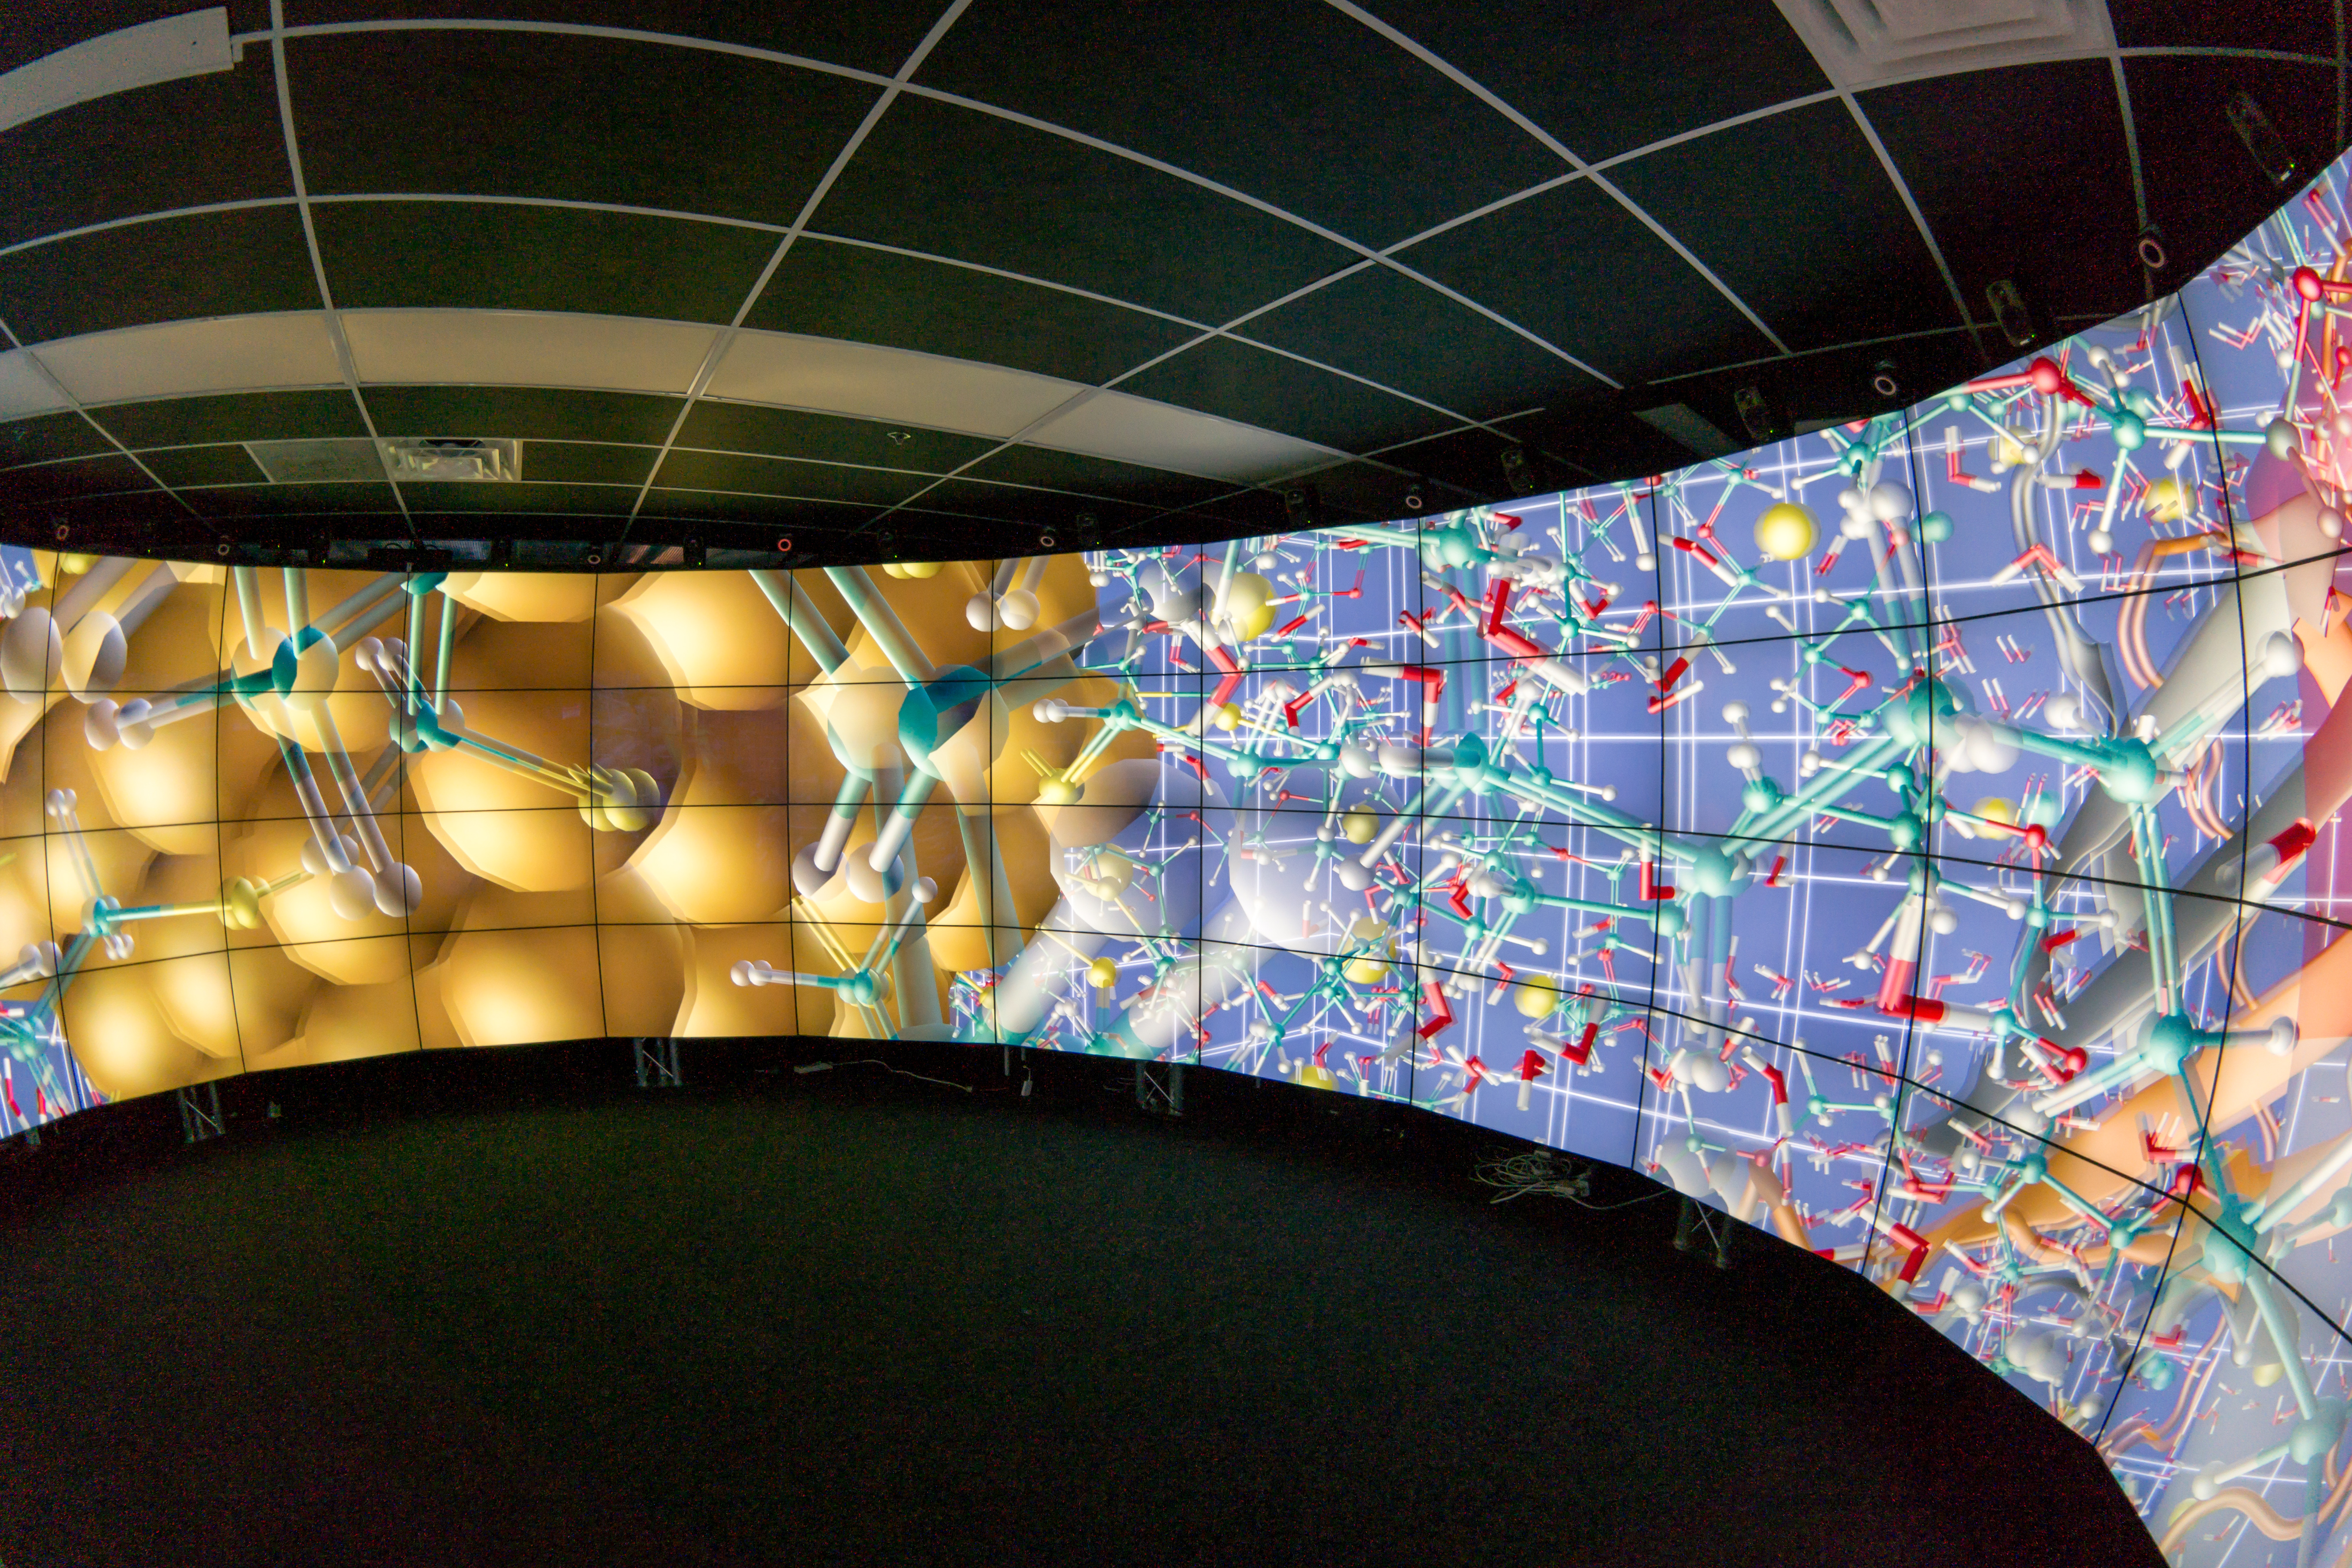
\includegraphics[height=5cm]{images/cave2}\\%
 \includegraphics[height=5.27cm]{images/cave}\hfil%
 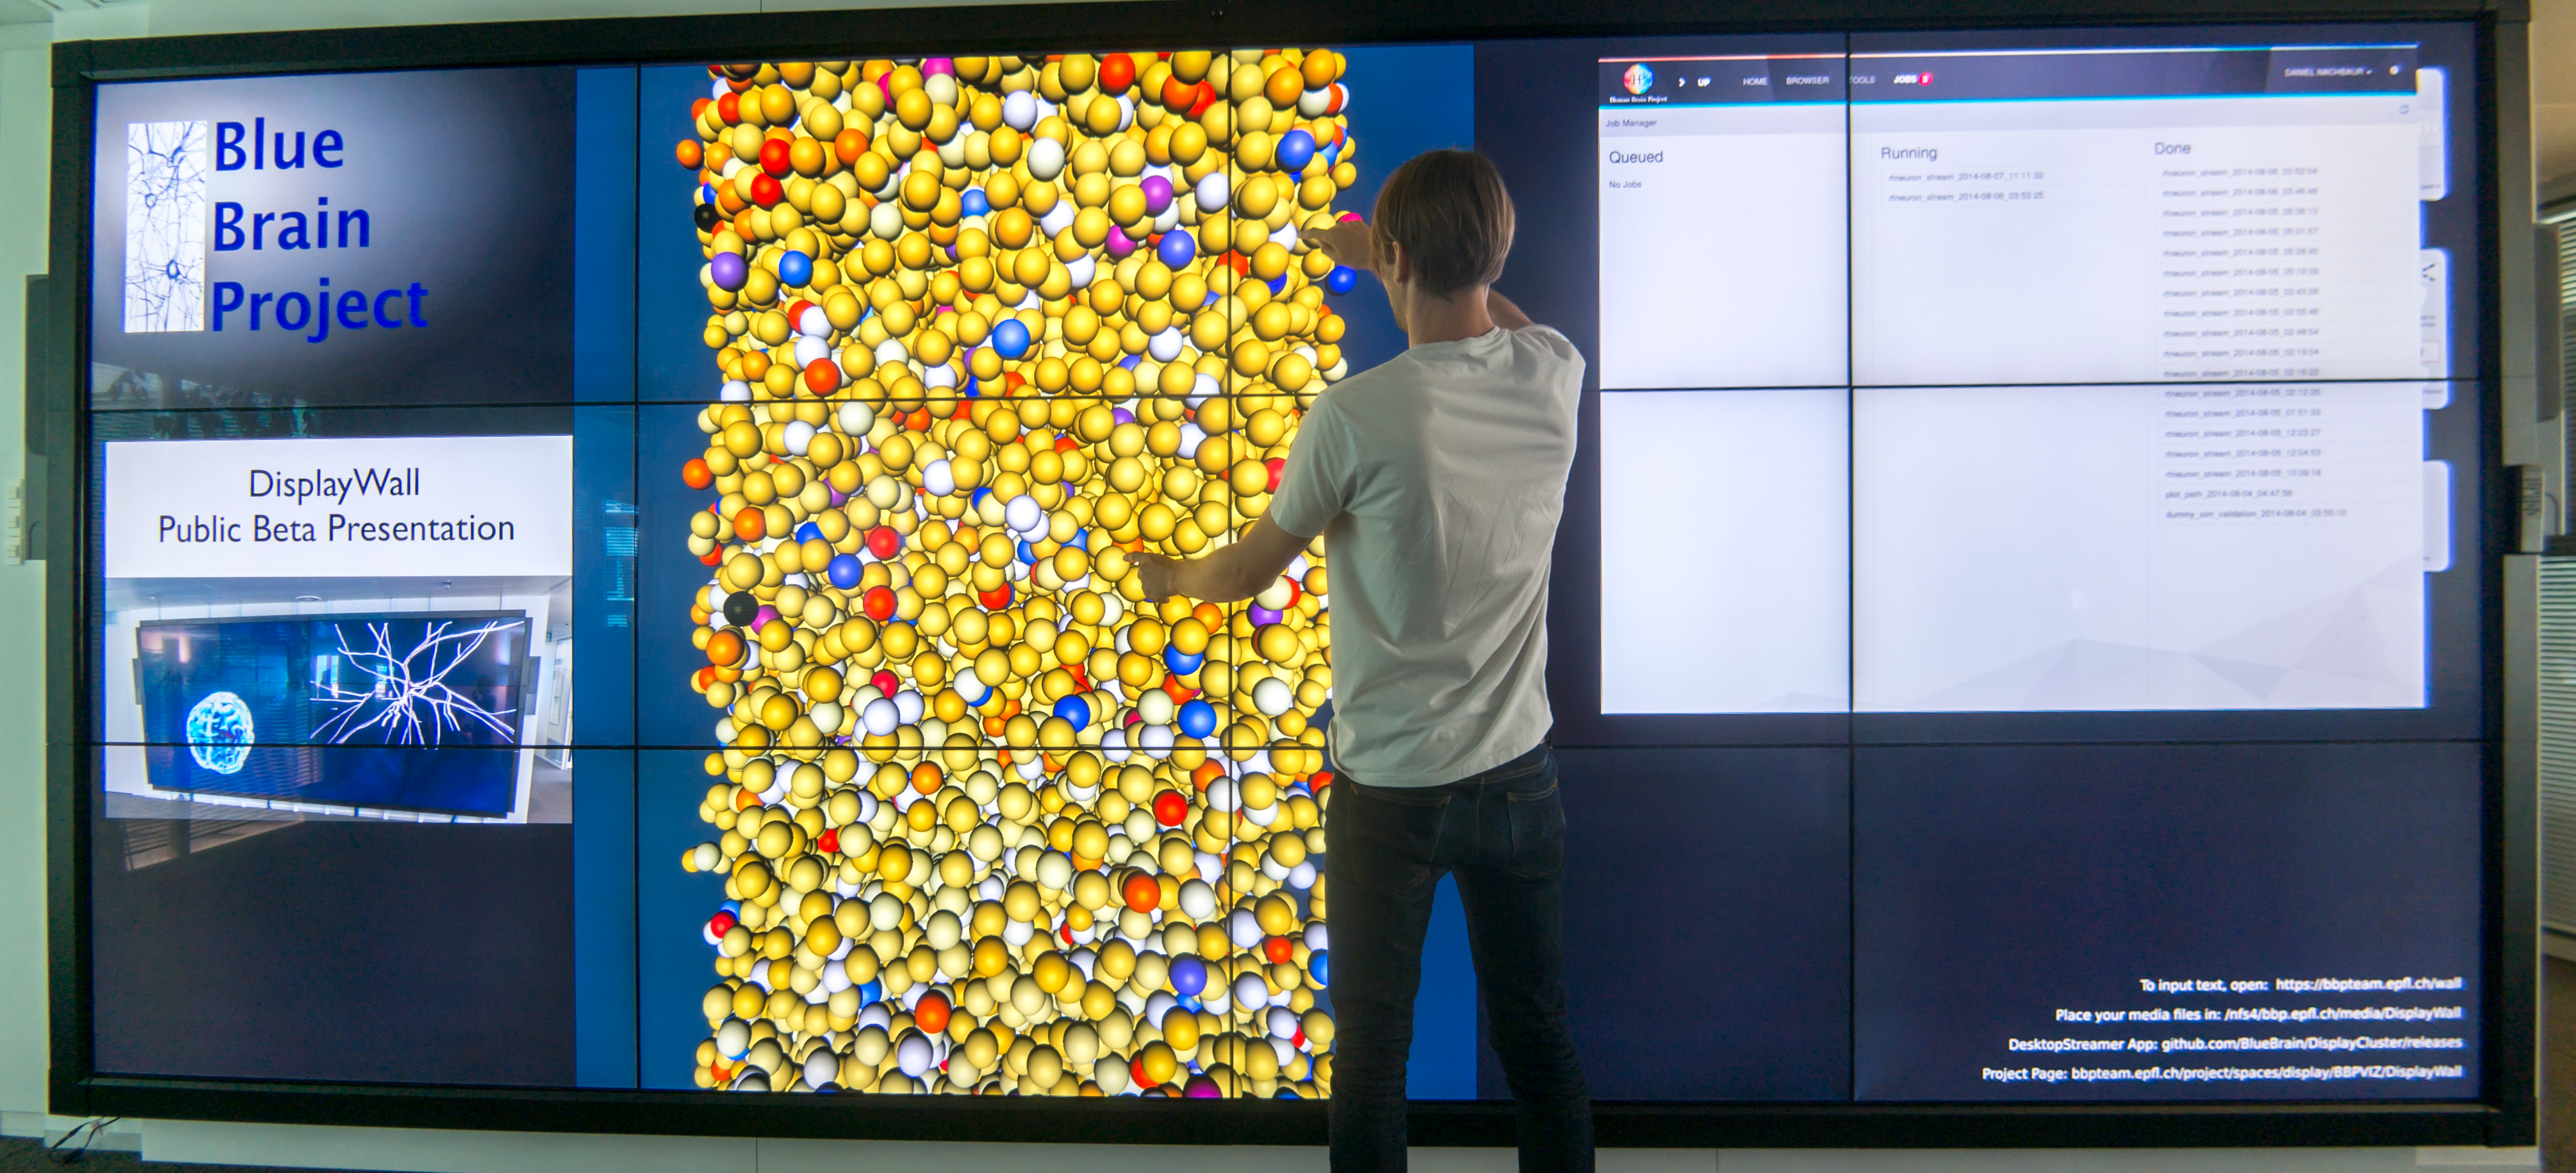
\includegraphics[height=5.27cm]{images/tide}%
 \caption{Large Data Visualization: Large data visualization of a
  brain simulation, molecular visualization in the Cave$^2$, exploration of EM
  stack reconstructions in a Cave, collaborative data analysis on a tiled
  display wall.}
\end{figure}

Display technology has made significant progress in the last decade.
High-resolution screens and tiled display walls are now affordabe for most
organizations and are getting deployed at an increasing rate. This increased
resolution and display size helps with understanding the data, but with the
quadratic increase in pixels to be rendered, it increases the pressure on
rendering algorithms to deliver interactive framerates. Furthermore, for larger
system it becomes necessary to develop parallel and distributed applications.

However, not only applications are becoming more and more data-driven, but also
the technology used to tackle these kinds of problems is rapidly witnessing a
paradigm shift towards massively parallel on-chip and distributed parallel
cluster solutions. On one hand, parallelism within a system has increased
massively, with tenths of CPU cores, thousands of GPU cores and multiple CPUs
and GPUs in a single system. On the other hand, massively parallel distributed
systems are easily accessible from various cloud infrastructure providers, and
are also affordable for on-site hosting for many organizations.

System software to exploit the available hardware parallelism capable of
performing efficient interactive data exploration has not kept up with the pace
in hardware developments and data gathering capabilities. On one hand, this is
due to an inherent delay between hardware and software capabilities, since
development typically only starts once the hardware is available. On the other
hand, existing software engineered for different design parameters has a
significant inertia to change, to the extreme of the necessity to rewrite it
from scratch.

In the context of emerging data-intensive knowledge discovery and data analysis,
efficient interactive data exploration methodologies have become increasingly
important. Visual analysis by means of interactive visualization and inspection
of three-dimensional data is a particularly efficient approach to gain intuitive
insight into the spatial structure and relations of very large 3D data sets.
However, defining visual and interactive methods scalable with problem size and
degree of parallelism, as well as generic applicability of high-performance
interactive visualization methods and systems are recognized among the major
current and future challenges.

\section{Interactive Visualization}

\section{Parallel Rendering}

The main performance indicator for Large Data Interactive Rendering is the
performance of the rendering algorithm, that is, the framerate with which the
program produces new images. This framerate can be improved by either using
faster or more hardware, or by better algorithms exploiting the existing
hardware and data. This proposal primarily focuses on the first approach using
parallel rendering to exploit the CPU and GPU parallelism available on a single
system or a distributed cluster.  The early fundamental concepts have been laid
down in \cite{MCEF:94} and \cite{Crockett:97}. A number of domain specific
parallel rendering algorithms and special-purpose hardware solutions have been
proposed in the past, however, only few generic parallel rendering frameworks
have been developed (\fig{fSorts}). We will focus on sort-last and sort-first
rendering, since sort-middle architectures are only feasible in a hardware
implementation due to the large amount of fragments processed and transferred in
the sorting stage.

\begin{figure}[ht]\center
 \includegraphics[width=0.7\textwidth]{images/all_sorts}%
 \caption{Sort-last, sort-middle and sort-first parallel rendering\label{fSorts}}
\end{figure}


\subsection{Domain specific solutions}

Cluster-based parallel rendering has been commercialized for off-line rendering
(i.e. distributed ray-tracing) for computer generated animated movies or special
effects, since the ray-tracing technique is inherently amenable to
parallelization for off-line processing. Other special-purpose solutions exist
for parallel rendering in specific application domains such as volume rendering
\cite{LWMT:97,Wittenbrink:98,HSCSM:00,SL:02,GS:02,NSJLYZ:05} or
geo-visualization \cite{VR:91,AG:95,LDC:96,JLMV:06}. However, such specific
solutions are typically not applicable as a generic parallel rendering paradigm
and do not translate to arbitrary scientific visualization and distributed
graphics problems.

In \cite{NC:07}, parallel rendering of hierarchical level-of-detail (LOD) data
has been addressed and a solution specific to sort-first tile-based parallel
rendering has been presented. While the presented approach is not a generic
parallel rendering system, basic concepts presented in \cite{NC:07} such as load
management and adaptive LOD data traversal can be carried over to other
sort-first parallel rendering solutions.

\subsection{Special-purpose architectures}

Historically, high-performance real-time rendering systems have relied on an
integrated proprietary system architecture, such as the early SGI graphics super
computers. These special-purpose solutions have become a niche product as their
graphics performance does not keep up with off-the-shelf workstation graphics
hardware and scalability of clusters.

Due to its conceptual simplicity, a number of special-purpose image compositing
hardware solutions for sort-last parallel rendering have been developed. The
proposed hardware architectures include Sepia \cite {MHS:99a,sepia}, Sepia~2
\cite{LMSBHa:01,LMSBH:01}, Lightning~2 \cite{Stoll01}, Metabuffer
\cite{Blanke00,Zhang01}, MPC Compositor \cite{Muraki01} and PixelFlow
\cite{Molnar92,Eyles97}, of which only a few have reached the commercial
product stage (i.e. Sepia~2 and MPC Compositor). However, the inherent
inflexibility and setup overhead have limited their distribution and application
support. Moreover, with the recent advances in the speed of CPU-GPU interfaces,
such as PCI Express, NVLink and other modern interconnects, combinations of
software and GPU-based solutions offer more flexibility at comparable
performance.

\subsection{Generic approaches}

A number of algorithms and systems for parallel rendering have been developed in
the past. On one hand, some general concepts applicable to cluster parallel
rendering have been presented in \cite{Mueller:95,Mueller:97} (sort-first
architecture), \cite{SZFLS:99,SFLS:00} (load balancing), \cite{SFL:01} (data
replication), or \cite{CMF:05,CM:06} (scalability). On the other hand, specific
algorithms have been developed for cluster based rendering and compositing such
as \cite{AP:98}, \cite{CKS:02} and \cite{YYC:01,SMLAP:03}. However, these
approaches do not constitute APIs and libraries that can readily be integrated
into existing visualization applications, although the issue of the design of a
parallel graphics interface has been addressed in \cite{Igehy98}.

Only few generic APIs and (cluster-)parallel rendering systems exist which
include VR Juggler \cite{BJHMBC:01} (and its derivatives), Chromium
\cite{HHNFAKK:02} (an evolution of \cite{Humphreys99,Humphreys00,HEBSEH:01}),
{ClusterGL}~\cite{NHM:11} and OpenGL Multipipe SDK
\cite{JDBJBCER:04,BRE:05,MPK}. These approaches can be categorized into
transparent interception and distribution of the OpenGL command stream and into
the parallization of the application rendering code (\fig{fChromium}).

\begin{figure}[ht]
 \includegraphics[height=4cm]{images/Chromium}\hfil%
 \includegraphics[height=4cm]{images/MPK}%
 \caption{Transparent OpenGL interception and parallelization of the rendering code\label{fChromium}}
\end{figure}


VR Juggler \cite{BJHMBC:01,JBBC:98} is a graphics framework for virtual reality
applications which shields the application developer from the underlying
hardware architecture, devices and operating system. Its main aim is to make
virtual reality configurations easy to set up and use without the need to know
details about the devices and hardware configuration, but not specifically to
provide scalable parallel rendering. Extensions of VR Juggler, such as for
example ClusterJuggler \cite{BC:03} and NetJuggler \cite{AGLMR:02}, are
typically based on the replication of application and data on each cluster node
and basically take care of synchronization issues, but fail to provide a
flexible and powerful configuration mechanism that efficiently supports scalable
rendering as also noted in \cite{SWNH:03}. VR Juggler does not support scalable
parallel rendering such as sort-first and sort-last task decomposition and image
compositing nor does it provide support for network swap barriers
(synchronization), distributed objects, image compression and transmission, or
multiple rendering threads per process, important for multi-GPU systems.

While Chromium \cite{HHNFAKK:02} provides a powerful and transparent abstraction
of the OpenGL API, that allows a flexible configuration of display resources,
its main limitation with respect to scalable rendering is that it is focused on
streaming OpenGL commands through a network of nodes, often initiated from a
single source. This has also been observed in \cite{SWNH:03}. The problem comes
in when the OpenGL stream is large in size, due to not only containing OpenGL
calls but also the rendered data such as geometry and image data. Only if the
geometry and textures are mostly static and can be kept in GPU memory on the
graphics card, no significant bottleneck can be expected as then the OpenGL
stream is composed of a relatively small number of rendering instructions.
However, as it is typical in real-world visualization applications, display and
object settings are interactively manipulated, data and parameters may change
dynamically, and large data sets do not fit statically in GPU memory but are
often dynamically loaded from out-of-core and/or multiresolution data
structures. This can lead to frequent updates not only of commands and
parameters wich have to be distributed but also of the rendered data itself
(geometry and texture), thus causing the OpenGL stream to expand dramatically.
Furthermore, this stream of function calls and data must be packaged and
broadcast in real-time over the network to multiple nodes for each rendered
frame. This makes CPU performance and network bandwidth a more likely limiting
factor.

The performance experiments in \cite{HHNFAKK:02} indicate that Chromium is
working quite well when the rendering problem is fill-rate limited. This is due
to the fact that the OpenGL commands and a non-critical amount of rendering data
can be distributed to multiple nodes without significant problems and since the
critical fill-rate work is then performed locally on the graphics hardware.

Chromium also provides some facilities for parallel application development,
namely a sort-last, binary-swap compositing SPU and an OpenGL extension
providing synchronization primitives, such as a barrier and semaphore. It leaves
other problems, such as configuration, task decomposition as well as process and
thread management unaddressed. Parallel Chromium applications tend to be written
for one specific parallel rendering use case, such as for example the sort-first
distributed memory volume renderer \cite{BHPB:03} or the sort-last parallel
volume renderer raptor \cite{Raptor}. We are not aware of a generic
Chromium-based application using many-to-one sort-first or stereo
decompositions.

The concept of transparent OpenGL interception popularized by WireGL and
Chromium has received some further contributions. While some commercial
implementations such as {TechViz} and {MechDyne Conduit} continue to exist, on
the research side only {ClusterGL}~\cite{NHM:11} has been presented recently.
{ClusterGL} employs the same approach as {Chromium}, but delivers a
significantly faster implementation of transparent OpenGL interception and
distribution for parallel rendering. Transparent OpenGL interception is an
appealing apporach for some applications since it requires no code changes, but
it has inherent limitiations due to the fact that eventually the bottleneck
becomes the single-threaded application rendering code, the amount of
application data the single application instance can load or process, or the the
size of the OpenGL command stream send over the network.

{CGLX}~\cite{DK:11} tries to bring parallel execution transparently to
OpenGL applications, by emulating the GLUT API and intercepting certain OpenGL
calls. In contrast to frameworks like {Chromium} and {ClusterGL}
which distribute OpenGL calls, {CGLX} follows the distributed application
approach. This works transparently for trivial applications, but quickly
requires the application developer to address the complexities of a distributed
application, when mutable application state needs to be synchronized across
processes. For realistic applications, writing parallel applications remains the
only viable approach for scalable parallel rendering, as shown by the success of
 {Paraview}, {Visit} and {Equalizer}-based applications.

OpenGL Multipipe SDK (MPK) \cite{BRE:05} implemented an effective parallel
rendering API for a shared memory multi-CPU/GPU system. It is similar to IRIS
Performer \cite{RH:94} in that it handles multi-GPU rendering by a lean
abstraction layer via a conceptual callback mechanism, and that it runs
different application tasks in parallel. However, MPK is not designed nor meant
for rendering nodes separated by a network. MPK focuses on providing a parallel
rendering framework for a single application, parts of which are run in parallel
on multiple rendering channels, such as the culling, rendering and final image
compositing processes.

Software for driving and interacting with tiled display walls has received
significant attention, including {Sage}~\cite{Sage} and
 {Sage~2}~\cite{Sage2} in particular. {Sage} was built entirely
around the concept of a shared framebuffer where all content windows are
separate applications using pixel streaming but is no longer actively supported.
{Sage 2} is a complete, browser-centric reimplementation where each
application is a web application distributed across browser instances.
{DisplayCluster}~\cite{DisplayCluster}, and its continuation
 {Tide}~\cite{tide}, also implement the shared framebuffer concept of
 {Sage}, but provide a few native content applications integrated into the
display servers. These solutions implement a scalable display environment and
are a target display platform for scalable 3D graphics applications.

\section{Dissertation Structure}


\chapter{Contributions}

Features, papers, individual contribution per paper.

\section{Generic Parallel Rendering Framework}

\section{Parallel Rendering Modes}

\section{Load Balancing}

\section{Applications}


\chapter{Parallel Rendering Framework Architecture}

\section{Overview}
A generic parallel rendering framework has to cover a wide range of use cases,
target systems, and configurations. This requires on one hand a strong
separation between the implementation of an application and its configuration,
and on the other hand a careful design to allow the resulting program to scale
up to hundreds of nodes, while providing a minimally invasive API for the
developer. In this section we present the system architecture of the Equalizer
parallel rendering framework, and motivate its design in contrast to related
work.

The motivation to use parallel rendering is either driven by the need to drive
multiple displays or projectors from multiple GPUs and potentially multiple
nodes, or by the need to increase rendering performance to be able to visualize
more data or use a more demanding rendering algorithm for higher visual quality.
Occasionally both needs coincide, for example for the analysis for large data
sets on high fidelity visualization systems.

Fundamentally, there are two approaches to enable applications to use multiple
GPUs: transparent interception at the graphics API (typically OpenGL) or
extending the application to support parallel rendering natively. The first
approach has been extensively explored by Chromium and others, while the second
is the foundation for this thesis. The architecture of Equalizer is founded on
an in-depth requirements analysis of typical visualization applications,
existing frameworks, and previous work on OpenGL Multipipe SDK.

The task of parallelizing a visualization application boils down to configuring
the application's rendering code differently for each resource, enabling this
rendering code to access the correct data, and synchronizing execution. For
scalable rendering, when multiple GPUs are used to accelerate a single output,
partial results need to be collected from all contributing resources and
combined on the output. Equalizer has a strong seperation of the rendering code
from its runtime configuration. The configuration is layed out in a hierarchical
resource description and compound trees configuring the resources for parallel
and scalable rendering. The configuration is a dynamic runtime structure, with a
serialized configuration file format.

In the following we will first describe the execution model and runtime
configurability, followed by the how the generic configuration is used to model
the desired visualization setup, and finally introduce specifics of scalable and
distributed rendering.

\section{Asynchronous Execution Model}

The core execution model for parallel rendering was pioneered by CAVELib
\cite{DACNCCGHPSNS:97}, refined by OpenGL Multipipe SDK for shared memory
systems and scalable rendering, and substantially extended by Equalizer for
asynchronous and distributed execution. By analysing the typical architecture of
a visualization application we observe an initialization phase, a main rendering
loop, and an exit phase. Equalizer decomposes these steps for parallel
execution.

The main rendering loop typically consists of four phases: submitting the
rendering commands to the graphics subsystem, displaying the renderered image,
and retrieving events from the operating system, based on which the application
state is updated and a new image is rendered. The configuration of the rendering
is largely hard-coded, with a few configurables such as field of view or stereo
separation. For parallel execution, we need to separate the rendering code from
this main loop, and execute it in parallel with different rendering parameters,
as shown in \fig{FIG_execution}. Similarly, the initialization and exit phase
also needs to be decomposed to allow managing multiple, distributed resources.

\begin{figure}[ht]\center
 \includegraphics[width=.9\columnwidth]{images/executionFlow}
 \caption{Simplified execution flow of a classical visualization application
  and an Equalizer application.}
 \label{FIG_execution}
\end{figure}

Without going into the details at this point, another critical design parameter
are synchronization points. Most implementations use a per-frame barrier or
similar synchronization to manages parallel execution. In larger installations,
this is detrimental for scalability, as even slight load imbalances limit
parallel speedup. The Equalizer execution model is fully asynchronuous, and only
introduces synchronization points when strictly needed. The main synchronization
points are: configured swap barriers between a set of output which have to
display simultaneously, the availability of input frames for scalable rendering,
and a task synchronization to prevent runaway of the main loop execution. By
default, Equalizer keeps up to one frame of latency in execution, that is, some
resource might render the next frame while others are still finishing the
current. Nonetheless, resources which are ready will immediately display their
result. The asynchronous execution architecture, coupled with a frame of
latency, allows pipelining of many operations, such as the application event
processing, task computation and load balancing, rendering, image readback,
compression, network transmission, and compositing.

\fig{fSyncAsync} shows the execution of the rendering tasks of a 2-node
sort-first compound without latency and with a latency of one frame. The
asynchronous execution pipelines rendering operations and hides imbalances in
the load distribution, resulting in an improved framerate. For example, we have
observed a speedup of 15\% on a five-node rendering cluster when using a latency
of one frame instead of no latency.

\begin{figure}[ht!]\center
 \includegraphics[width=\textwidth]{images/syncAsync}
 {\caption{\label{fSyncAsync}Synchronous and Asynchronous Execution}}
\end{figure}


\subsection{Programming Interface}

Equalizer provides a framework to facilitate the development of distributed as
well as non-distributed parallel rendering applications. The programming
interface is based on a set of C++ classes, modeled closely to the resource
hierarchy of a graphics rendering system. The application subclasses these
objects and overrides C++ task methods, similar to C callbacks. These task
methods will be called in parallel by the framework, depending on the current
configuration. This parallel rendering interface is significantly different from
Chromium \cite{HHNFAKK:02} and more similar to VRJuggler \cite{BJHMBC:01} or
OpenGL Multipipe SDK \cite{BRE:05}.

\begin{wrapfigure}{r}{.618\textwidth}
 \includegraphics[width=.618\textwidth]{images/processes}
 {\caption{\label{fProcessing}Parallel Rendering Entities}}
\end{wrapfigure}

To separate the responsibilities in a parallel rendering application, different
entities are resonsible for different aspects of the runtime system: the
application process to drive a rendering session, the server process or thread
to control the parallel rendering configuration, render clients to execute the
rendering tasks, and an administrative API to reconfigure the rendering session
at runtime.

\subsection{Application}

The main application thread in Equalizer drives the rendering, that is, it
carries out the main rendering loop, but does not actually execute any
rendering. Depending on the configuration, the application process often hosts
one or more render client threads. When a configuration has no additional nodes
besides the application node, all application code is executed in the same
process, and no network data distribution has to be implemented. The main
rendering loop is quite simple: The application requests a new frame to be
rendered, synchronizes on the completion of a frame and processes events
received from the render clients. Figure~\ref{FIG_execution} shows a simplified
execution model of an Equalizer application.


\subsection{Server}

The Equalizer server manages the parallel rendering session. It is an
asynchronous execution thread or process which receives requests from the
application and serves these requests using the current configuration, launching
and stopping rendering client processes on nodes, determining the rendering
tasks for a frame, and synchronizing the completion of tasks.

\subsection{Render Client}

During initialization of the server, the application provides a rendering client
executable. The rendering client is often, especially for simple applications,
the same executable as the application. However, in more sophisticated
implementations the rendering client can be a smaller executable which only
contains the application-specific rendering code. The server deploys this
rendering client on all nodes specified in the configuration.

In contrast to the application process, the rendering client does not have a
main loop and is completely controlled by the Equalizer framework based on
application's commands. A render client consists of the following threads: the
node main thread, one network receive thread, and one thread for each graphics
card (GPU) to execute rendering tasks. If a configuration also uses the
application node for rendering, then the application process uses one or more
render threads, consistent with render client processes.

The Equalizer client library implements the main loop, which receives network
events, processes them, and invokes the necessary task methods provided by the
developer.

The task methods clear the frame buffer as necessary, execute the OpenGL
rendering commands as well as readback, and assemble partial frame results for
scalable rendering. All tasks have default implementations so that only the
application specific methods have to be implemented, which at least involves the
 {\tt frameDraw()} method executing a rendering task. For example, the default
callbacks for frame recomposition during scalable rendering implement tile-based
assembly for sort-first and stereo decompositions, and $z$-buffer compositing
for sort-last rendering.

\subsubsection{Render Context}

The render context is the core entity abstracting the application-specific
rendering algorithm from the system-specific configuration. It specifies:

\begin{compactdesc}
 \item[Buffer] OpenGL-style read and draw buffer as well as color mask.
 These parameters are influenced by the current eye pass, eye
 separation and anaglyphic stereo settings.
 \item[Viewport] Two-dimensional pixel viewport restricting the
 rendering area. For correct operations, both
 \textsf{glViewport} and \textsf{glScissor} have to be used. The pixel
 viewport is influenced by the destination viewport
 definition and viewports set for sort-first/2D decompositions.
 \item[Frustum] Frustum parameters as defined by
 \textsf{glFrustum}. Typically the frustum used to set up the OpenGL projection
 matrix. The frustum is influenced by the destination's view
 definition, sort-first decomposition, tracking head matrix and the current eye pass.
 \item[Head Transformation] A transformation matrix positioning the frustum. For
 planar views this is an identity matrix and is used in immersive rendering.
 It is normally used to set up the `view' part of the modelview matrix, before
 static light sources are defined.
 \item[Range] A one-dimensional range with the interval [0..1]. This parameter is
 optional and should be used by the application to render only the appropriate
 subset of its data for sort-last rendering.
\end{compactdesc}

\subsubsection{Event Handling}

Event handling routes events from the source (the window in the rendering
thread) gradually to the the application main thread for consumption. At each
step, events can be observed, transformed or dropped. Events are received from
the operating system in the rendering thread, transformed there into a generic
representation, and sent over the network to the application. The application
processes them in the main loop and modifies its internal state accordingly.


\section{Configuration}

A configuration consists of the declaration of the rendering (hardware)
resources, the physical and logical  description of the projection system, and
the description on how the  aforementioned resources are used for parallel and
scalable rendering.

The rendering resources are represented in a hierarchical tree structure
which corresponds to the physical and logical resources found in a 3D
rendering environment: nodes (computers), pipes (graphics cards),
windows, and channels.

Physical layouts of display systems are configured using canvases with
segments, which represent 2D rendering areas composed of multiple
displays or projectors. Logical layouts are applied to canvases and
define views on a canvas.

Scalable resource usage is configured using a compound tree, which is a
hierarchical representation of the rendering decomposition and
recomposition across the resources.

\subsection{Rendering Resources}

The first part of the configuration is a hierarchical structure of
nodes-pipes-win\-dows-channels describing the rendering resources. The developer
will use instances of these classes to implement application logic and manage
data.

The \textsf{node} is the representation of a single computer in a cluster. One operating
system process of the render client executable will be used for each node. Each
configuration might also use an application node, in which case the application
process is also used for rendering. All node-specific task methods are executed
from the main thread.

The \textsf{pipe} is the abstraction of a graphics card (GPU), and uses an
operating system thread for rendering. All pipe, window and channel task methods
are executed from the pipe thread. The pipe maintains the information about the
GPU to be used by the windows for rendering.

The \textsf{window} encapsulates a drawable and an OpenGL context. The drawable
can be an on-screen window or an off-screen pbuffer or framebuffer object (FBO).
Windows on the same pipe share their OpenGL rendering resources. They execute
their rendering tasks sequentially on the pipe's execution thread.

The \textsf{channel} is the abstraction of an OpenGL viewport within its parent
window. It is the entity executing the actual rendering. The channel's viewport
is overwritten when it is rendering for another channel during scalable
rendering. Multiple channels in application windows may be used to view the
model from different viewports. Sometimes, a single window is split across
multiple projectors, e.g., by using an external splitter such as the Matrox
TripleHead2Go.


\subsection{Display Resources}

Display resources are the second part of a configuration. They describe the
physical display setup (canvases-segments), logical display (layouts-views) and
head tracking of users within the visualization installation (observers).

A \textsf{canvas} represents one physical projection surface, e.g., a PowerWall,
a curved screen or an immersive installation. Canvases provide a convenient way
to configure projection surfaces. A canvas uses layouts, which describe logical
views. Typically, each desktop window uses one canvas, one segment, one layout
and one view. One configuration might drive multiple canvases, for example an
immersive installation and an operator station. Planar surfaces, e.g., a display
wall, configure a frustum for the respective canvas. For non-planar surfaces,
the frustum will be configured on each display segment.

\begin{wrapfigure}{r}{.618\textwidth}
 \includegraphics[width=.618\textwidth]{images/frusta.pdf}
 {\caption{\label{fFrusta}Wall and Projection Parameters}}
\end{wrapfigure}

The frustum can be specified as a wall or projection description in the same
reference system as used by the head-tracking matrix calculated by the
application.  A wall is completely defined by the bottom-left, bottom-right and
top-left coordinates relative to the origin.  A projection is defined by the
position and head-pitch-roll orientation of the projector, as well as the
horizontal and vertical field-of-view and distance of the projection wall.
\fig{fFrusta} illustrates the wall and projection frustum parameters.

A canvas consists of one or more segments. A planar canvas typically has a
frustum description (see \sref{sFrustum}), which is inherited by the segments.
Non-planar frusta are configured using the segment frusta. These frusta
typically describe a physically correct display setup for Virtual Reality
installations.

A canvas has one or more layouts. One of the layouts is the active
layout, that is, this set of views is currently used for rendering. It
is possible to specify \textsf{OFF} as a layout, which deactivates the
canvas. It is possible to use the same layout on different canvases.

\begin{wrapfigure}{r}{.382\textwidth}
 \includegraphics[width=.382\textwidth]{images/canvas.pdf}
 {\caption{\label{fCanvas}A Canvas using four Segments}}
\end{wrapfigure}

A \textsf{segment} represents one output channel of the canvas, e.g., a
projector or a display. A segment has an output channel, which references the
channel to which the display device is connected. To synchronize the video
output, a canvas swap barrier or a swap barrier on each segment synchronize the
respective window buffer swaps.

A segment covers a part of its parent canvas, which is configured using the
segment viewport. The viewport is in normalized coordinates relative to the
canvas. Segments might overlap (edge-blended projectors) or have gaps between
each other (display walls, \fig{fCanvas}\footnote{Dataset courtesy of VolVis
 distribution of SUNY Stony Brook, NY, USA.}). The viewport is used to
configure the segment's default frustum from the canvas frustum description, and
to place layout views correctly.

A \textsf{layout} is the grouping of logical views. It is used by one or more
canvases. For all given layout/canvas combinations, Equalizer creates
destination channels when the configuration file is loaded. These destination
channels are later referenced by compounds to configure scalable rendering.
Layouts can be switched at runtime by the application. Switching a layout will
activate different destination channels for rendering.

\begin{wrapfigure}{r}{.618\textwidth}
 \includegraphics[width=.618\textwidth]{images/layout.png}
 {\caption{\label{fLayout}Layout with four Views}}
\end{wrapfigure}

A \textsf{view} is a logical view of the application data, in the sense used by
the Model-View-Controller pattern. It can be a scene, viewing mode, viewing
position, or any other representation of the application's data. A view has a
fractional viewport relative to its layout. A layout is often fully covered by
its views, but this is not a requirement. Each view can have a frustum
description. The view's frustum overrides frusta specified at the canvas or
segment level. This is typically used for non-physically correct rendering,
e.g., to compare two models side-by-side on a canvas. If the view does not
specify a frustum, it will use the sub-frustum resulting from the covered area
on the canvas.

A view might have an observer, in which case its frustum is tracked by this
observer. \fig{fLayout} shows an example layout using four views on a single
segment. \fig{fDisplay} shows a real-world setup of a single canvas with six
segments using underlap, with a two-view layout activated. This configuration
generates eight destination channels.

\begin{figure}[ht!]\center
 \includegraphics[width=.9\textwidth]{images/wallLayout.jpg}
 {\caption{\label{fDisplay}Display Wall using a six-Segment Canvas with a two-View Layout}}
\end{figure}

An \textsf{observer} represents an actor looking at multiple views. It has a
head matrix, defining its position and orientation within the world, an eye
separation and focus distance parameters. Typically, a configuration has one
observer. Configurations with multiple observers are used if multiple,
head-tracked users are in the same configuration session, e.g., a non-tracked
control host with two tracked head-mounted displays.

\subsection{Compounds}

Compound trees are used to describe how multiple rendering resources are
combined to produce the desired output, especially how multiple GPUs are
aggregated to increase rendering performance. They are the core contribution
enabling a flexible resource configuration.

Compounds are a data structure to describe the parallel execution of rendering
tasks in the form of a tree.  Each compound corresponds to some rendering tasks
(clear, draw, assemble, readback) and references a  channel from the resource
description which executes the tasks in the given order. A compound may provide
output frames from the readback task to others, and can request input
frames from others for its own assembly task, and output frames are linked to
input frames by name.

Compound trees are a logical description of the rendering pipeline, and only
reference the actual physical resources through their channels. This allows
mapping a compound tree to different physical configurations by simply replacing
the channel IDs. For example, one can test the functionality of a sort-last
configuration by using channels of different windows on one local workstation
before deploying it to multiple physical GPUs.

A simple leaf compound description for rendering a part of the data set, given
by the data {\em range}, into a particular region of the {\em viewport} is given
in \fig{FIG_leaf_compound}. The data range is a logical mapping of the data set
onto the unit interval and is left to the application to interpret
appropriately. Hence  the range [0 $\frac{1}{2}$] indicates that the first half
of the data set should be rendered, for example the first $\frac{n}{2}$
triangles of a polygonal mesh with $n$ faces. The viewport is indicated by the
parameters [x y width height] as fraction of the parent's viewport, and in the
example the data is thus rendered into the left half of the viewport. The
resulting framebuffer data -- including per-pixel color and depth -- of the
rendering executed on this channel is read back and made available to other
compounds by the name left\_half.

\begin{figure}[ht]\center
 {\begin{tabbing} \ \ \ \ \ \=\ \ \ \=\ \ \ \=\ \ \ \=\ \ \ \=\ \ \ \= \kill
   \> {\bf compound} \{						\\
   \>\> {\bf channel} "draw"					\\
   \>\> buffer  [ COLOR DEPTH ]				\\
   \>\> range [0 $\frac{1}{2}$]				\\
   \>\> viewport [ 0 0 $\frac{1}{2}$ 1 ]                 \\
   \>\> outputframe \{name "left\_half" \}	\\
   \> \}
  \end{tabbing}}
 \vspace{-2mm}
 \caption{Compound executing rendering of a part of the data set into a given region of the viewport.\label{FIG_leaf_compound}}
\end{figure}

A non-leaf compound performing some image assembly and compositing task is
indicated in \fig{FIG_inner_compound}. Framebuffer data is read from two other
compounds which supposedly execute rendering for part\_a and part\_b of the data
set in parallel. The compound itself executes for example $z$-depth visibility
compositing of the two input images on its channel and returns the resulting
color framebuffer.

\begin{figure}[ht]\center
 {\begin{tabbing} \ \ \ \ \ \=\ \ \ \=\ \ \ \=\ \ \ \=\ \ \ \=\ \ \ \= \kill
   \> {\bf compound} \{						\\
   \>\> {\bf channel} "display"				\\
   \>\> inputframe \{ name "part\_a" \}			\\
   \>\> inputframe \{ name "part\_b" \}			\\
   \>\> outputframe \{ buffer [ COLOR ] \}	\\
   \> \}
  \end{tabbing}}
 \vspace{-2mm}
 \caption{Compound performing image compositing.\label{FIG_inner_compound}}
\end{figure}

Leaf compounds execute all tasks by default, but the focus is often on the draw
task with a default assemble and standard readback task used to pass the
resulting image data on to other compounds for further compositing. Hence while
leaf compounds execute the rendering in parallel, non-leaf compounds often
correspond to, but are not restricted to the (parallel) image compositing and
assembly part. The readback or assemble tasks are only active if output or input
frames have been specified, respectively. Otherwise the rendered image frame is
left in-place for further processing in a parent compound sharing the same
channel.

Note that non-leaf nodes in the compound tree structure traverse their children
first before performing their default assemble and readback tasks. Furthermore,
compounds only define the logical task decomposition structure, while its
execution is actually performed on the referenced channels. Therefore, since
compounds can share channels, as often done between a parent and one of its
child compounds, rendered image data can sometimes be left in place, avoiding
readback and transfer to another node.

All attributes as well as the channel are inherited from the parent compound if
not specified otherwise. The {\em viewport}, {\em data range} and {\em eye}
attributes are used to describe the decomposition of the parent's 2D viewport,
database range and eye passes, respectively.

A more formal classification of compound entities is:

\begin{compactdesc}
 \item [Root compound] is the top-level compound of a compound tree. It might
 also be a destination compound, or can be empty (not referencing a channel)
 when synchronizing multiple destination channels.
 \item [Destination compound(s)] are the top-most compound referencing a
 destination channel. This destination channel determines the rendering context
 for the whole subtree, that is, compounds and their channels lower in the
 hierarchy contribute to the rendering of the destination channel be executing
 part of the destination render context and providing output frames which will
 eventually be composited onto the destination channel.
 \item [Source compounds] are the leaf nodes in a compound tree. They typically
 use a different channel from the destination channel and configure scalability
 by overriding render context parameters. This decomposes the rendering of the
 destination channel. By adding output and input frames, the partial results are
 collected and composited:
 \begin{compactdesc}
  \item[Decomposition] On each child compound the rendering task of that
  child can be limited by setting the \textsf{viewport}, \textsf{range},
  \textsf{period} an  \textsf{phase}, \textsf{pixel}, \textsf{subpixel},
  \textsf{eye} or \textsf{zoom} as desired.
  \item[Compositing] Source compounds define an \textsf{output\_frame} to read
  back the result. This output frame is used as an \textsf{input\_frame} on the
  destination compound receiving the pixels. The frames are connected with each
  other by their name, which has to be unique within the root compound tree. For
  parallel compositing, the algorithm is described by defining multiple input
  and output frames across all source compounds.
 \end{compactdesc}
 \item[Intermediate compounds] may be used to simplify the task decompostion or
 to configure parallel compositing.
\end{compactdesc}

\section{Compositing}

In contrast to most other parallel rendering frameworks, Equalizer decouples the
compositing algorithm from the task decomposition. This is a critical component
in the architecture, allowing a flexible configuration, often in many unforeseen
ways. The compound tree with its task decomposition, input and output frames, is
a specialized description ``programming'' scalable rendering across parallel
resources.

Compositing if configured using output frames connected to input frames,
compound tasks and eye passes, as well as frame parameters. In its simplest
form, a sort-first source compound provides and output frame, which is routed to
an input frame using the same name on the destination compound. The source
viewport decomposes the task, and the output frame collects this partial result
from the source channel and composites it using the correct offset onto the
destination channel.

Frame parameters allow the customization of the pixel handling. They include the
transferred buffers (color, depth), partial channel viewport, and pixel zooming
(upscale and downscale). An output frame may be connected to multiple input
frames. These parameters are used in conjunction with compound tasks for
parallel compositing, and advanced features such as monitoring and dynamic frame
resolution introduced later.

\fig{fDirectSend} shows the pixel flow of direct send composting for a three-way
sort-last decomposition, where the destination channel also contributes to the
rendering. In the first step, each channel exchanges two color+depth tiles with
its neighbors, and then $z$-composites its own tile. This yields one complete
tile on each channel, of which two color tiles are then assembled on the
destination channel.

\begin{figure}[ht]
 \includegraphics[width=.57\textwidth]{images/directSend}
 \includegraphics[width=.42\textwidth]{images/directSendCompound}
 {\caption{\label{fDirectSend}Direct Send Compositing}}
\end{figure}

The corresponding compound tree is shown schematically on the right of
\fig{fDirectSend}. Each of the three channels has a child compound to execute
the rendering and read back to incomplete tiles for sort-last compositing. These
three leaf compounds represent the first step in the left-hand diagram. One
level up, each channel receives two tiles and assembles them onto its partially
rendered result, creating a complete tile. For the two source-only channels, a
final color-only output image is connected to the destination channel. The
arrows illustrate the pixel flow for one of the tiles.

For most rendering applications even a relatively complex setup such as this
example requires very little programmer involvement. The abstractions provided
by the resource description, render context and compounds enable Equalizer to
reconfigure the application almost transparently. For polygonal rendering, it
suffices that the application honors the \textsf{range} parameter of the render
context to decompose its rendering. All other tasks, in particular the parallel
compositing and pixel transfers, are fully handled by Equalizer. Applications
which require ordered compositing, for example volume rendering, overwrite the
assemble callback to reorder the input frames correctly.

The abstraction through frames is flexible, but still allows many architectural
optimizations:
\begin{compactdesc}
\item[Unordered Compositing:] Unless overwritten by the application, Equalizer
will composite all input frames in the order they become available, not in the
order they are configured. In the example from \fig{fDirectSend}, the
destination channel will assemble its four input frames one by one as the output
frame is received. Due to the asynchronous execution and resulting pipelining of
operations, this availability changes each frame depending on the runtime of
other tasks.
\item[Asynchronous Compression, GPU and Network Transfers:] Compressing,
transmitting and receiving frames between nodes is handled by threads
independent from the render thread. GPU transfers are handled by asynchronous
PBO transfers. Pipelining all these operations with the actual rendering
significantly minimizes the compositing overhead.
\item[On-GPU Transfers:] Occasionally, the source and destination channel are on
the same GPU. Using textures as pixel buffers allows minimal overhead for the
output to input frame transfer.
\end{compactdesc}

\section{Load Balancing}

Compounds in itself only provide a static configuration of the parallel
rendering setup. \textsf{Equalizers} are algorithms which hook into a compound
and modify parameters of their respective subtree at runtime to dynamically
optimize the resource usage, by each tuning one aspect of the decomposition. Due
to their nature, they are transparent to application developers, but might have
application-accessible parameters to tune their behavior. Resource equalization
is the critical component for scalable parallel rendering, and therefore the
eponym for the \textsf{Equalizer} project name.

Compounds are a static snapshot of a configuration, and equalizers provide
dynamic configuration on top. This separation of responsibilities is an
important architectural component of our parallel rendering framework. Load
balancing is one use case for equalizers, where the algorithm analysis runtime
statistics to change the task decomposition each frame to equalize rendering
times between all resources.

\section{Distributed Execution Layer}

An important part of writing a parallel rendering application is the
communication layer between the individual processes. \textsf{Equalizer} relies
on the \textsf{Collage} network library for its internal operation.
\textsf{Collage} provides networking functionality of different abstraction
layers, gradually providing higher level functionality for the programmer. The
main primitives in \textsf{Collage} and their relations are shown in
\fig{fNetObject} and provide:

\begin{compactdesc}
\item[Connection] A stream-oriented point-to-point communication
  line. Connections
  transmit raw data reliably between two endpoints for unicast connections, and
  between a set of endpoints for multicast connections. For unicast,
  process-local pipes, TCP and Infiniband RDMA are implemented. For multicast,
  a reliable, UDP-based protocol is discussed in \sref{sec:RSP}.
\item[DataI/OStream] Abstracts the marshalling of C++ classes from or to
  a set of connections by implementing output stream operators. Uses buffering
  to aggregate data for network transmission. Performs byte swapping during
  input if the endianness differs between the remote and local node.
\item[Node and LocalNode] The abstraction of a process in the cluster. Nodes
  communicate with each other using connections. A LocalNode listens on various
  connections and processes requests for a given process. Received data is
  wrapped in ICommands and dispatched to command handler methods. A Node is a
  proxy for a remote LocalNode.
\item[Object] Provides object-oriented, versioned data distribution of C++
  objects between nodes. Objects are registered or mapped on a Local\-Node.
\end{compactdesc}

\begin{figure}[ht]\center
  \includegraphics[width=\columnwidth]{images/netObject}
  \caption{\label{fNetObject}Communication between two \textsf{Collage} objects}
\end{figure}

\textsf{Collage} implements a few generic distributed objects which are used by
\textsf{Equalizer} and other applications. A barrier is a distributed barrier
primitive used for software swap synchronization. Its implementation follows a
simple master-slave approach, which has shown to by sufficient for this use
case. Queues are distributed, single producer, multiple consumer FIFO queues. To
hide network latencies, consumers prefetch items into a local queue. Queues are
used for tile and chunk compounds (\sref{sec:tile}).

An object map facilitates distribution and synchronization of a collection of
distributed objects. Master versions can be registered on a central node, e.g.,
the application node in \textsf{Equalizer}. Consumers, e.g., \textsf{Equalizer}
render clients, can selectively map the objects they are interested in.
Committing the object map will commit all registered objects and sync their new
version to the slaves. Syncing the map on the slaves will synchronize all mapped
instances to the new version recorded in the object map. This effective design
allows data distribution with minimal application logic.


\chapter{Scalable Rendering}

Scalable rendering is a subset of parallel rendering which aims to improve the
framerate of a rendering task by decomposing it over multiple rendering
resources. Parallel rendering includes other use cases, for example to use
multiple GPUs to drive individual displays of a tiled display wall.

Parallel rendering research has put a lot of focus on two of the three
architectures classified by \cite{Molnar92}: sort-first and sort-last rendering.
Sort-middle rendering is still largely confined to hardware implementations due
to its high communication cost of sorting and distributing fragments to
processing units.

In this chapter, we present a wide set of new parallelization schemes which
break out of this standard classification. For each mode, we present its
algorithm and implementation, potential impact on the application code, as well
as its strengths and weaknesses. Due to the flexible architecture of our
parallel rendering system, these modes are largely usable with any Equalizer
application and can be combined with all other modes.

Most of these rendering modes are similar to sort-first rendering, in that they
decompose the final view spatially or temporally. Stereo compounds decompose per
eye pass, DPlex compounds temporally, pixel and subpixel compounds use equal
spatial decompositions. Finally, tile and chunk compounds implement implicit
load-balancing for sort-first and sort-last rendering using queueing of work
items.

This wide set of decomposition modes for scalable rendering, embedded in our
generalized compound structure, enables applications and researchers to
decompose the rendering task in, as far as we know, any way possible for a
rendering pipeline. To our knowledge no other implementation provides this
breath and flexibility, and many of these algorithms appear for the first time
in Equalizer.

\section{Stereo}

Stereo, or eye decomposition, is a specialized version of sort-first rendering.
Two GPUs get assigned each one of the eye passes during stereo rendering. For
passive stereo, there is no compositing step needed, whereas for active and
anaglyphic stereo the frame buffer for one eye pass has to be copied to the
destination channel. Due to the strong similarity between both eye passes, this
mode provides close to perfect load balance. \fig{fStereo} shows an anaglyphic
stereo compound.

\begin{wrapfigure}{r}{.618\textwidth}
 \includegraphics[width=.618\textwidth]{images/Stereo}
 {\caption{\label{fStereo}Anaglyphic Stereo Compound}}
\end{wrapfigure}

While many implementations provide passive or active stereo rendering and
sometimes decomposition using two GPUs, our implementation within our flexible
compound structure allows to fully exploit stereo decomposition.  Stereoscopic
and monoscopic rendering is no special case in the architecture, but rather a
configuration of the rendering resources. Among other things, this allows
extending a two-way stereo decomposition with further resources and any other
scalable rendering mode. One can also easily set up an application with mixed
rendering, e.g., to render a monoscopic view on a control workstation while
rendering stereoscopic on a larger immersive installation.


\section{Time-Multiplex}

Time-multiplexing distributes full frames over the available resources, such
that each resource only renders a subset of the visible frames (\fig{fDPlex}).
This mode is also called alternate frame rate or DPlex, was first implemented in
\cite{BRE:05} for shared memory machines. The algorithm is however much better
suited for distributed memory systems, since the separate memory space makes
concurrent rendering of different frames much easier to implement. While it
increases the framerate almost linearly, it does not decrease the latency
between user input and the corresponding output. Consequently, this
decomposition mode is mostly useful for non-interactive movie generation.

\begin{wrapfigure}{r}{.382\textwidth}
\includegraphics[width=.382\textwidth]{images/DPlex}
{\caption{\label{fDPlex}Time-Multiplex Compound}} \end{wrapfigure}

DPlex is very well load-balanced, since most applications observe a strong
frame-to-frame coherence with respect to the rendering load. This decomposition
mode has the pecularity that small imbalances tend to accumulate such that the
concurrent frames all finish simultaneously. To provide a smooth framerate, if
so desired, a \textsf{framerate equalizer} can be installed on the destination
compound. \sref{sFramerateEq} covers this functionality. It is transparent to
\textsf{Equalizer} applications, but does require the configuration latency to
be equal or greater than the number of source channels.

DPlex rendering is not hard-coded into our framework, but configured by
restricting the rendering task temporally on each source compound. This is
achieved by setting a \textsf{period} and \textsf{phase} parameter, which
configure the number of frames skipped and starting offset on the given source
compound. A simple DPlex compound would have a destination compound with $n$
source compounds, where each source has a period of $n$ and one phase from
$0..n-1$. While this generalization may seem artificial, it opens up different
use cases, for example giving a fast GPU a smaller period, thus giving it more
work.

\section{Pixel}

\begin{wrapfigure}{r}{.382\textwidth}
 \includegraphics[width=.382\textwidth]{images/Pixel}
 {\caption{\label{fPixel}Pixel Compound}}
\end{wrapfigure}

Pixel compounds (\fig{fPixel}) decompose the destination channel by interleaving
pixels in image space. They are a variant of sort-first rendering which works
well for fill-limited applications which are not geometry bound, for example
direct volume rendering. Source channels cannot reduce geometry load through
view frustum culling, since each source channel has almost the same frustum.
However, the fragment load on all source channels is reduced linearly and well
load-balanced due to the interleaved distribution of pixels. This functionality
is transparent to \textsf{Equalizer} applications, and the default compositing
uses the stencil buffer to blit pixels onto the destination channel.

Pixel compounds are configured by restricting each source compound with a pixel
kernel. The kernel describes the size of the decomposition in 2D space, and the
2D pixel offset within this region. This follows our design philosophy of
enabling features by generalizing the underlying algorithm rather then
hardcoding them.

\section{Subpixel}

\begin{wrapfigure}{r}{.382\textwidth}
 \includegraphics[width=.382\textwidth]{images/Subpixel}
 {\caption{\label{fSubpixel}Subpixel Compound}}
\end{wrapfigure}

Subpixel compounds (\fig{fSubpixel}) are similar to pixel compounds, but they
decompose the work for a single pixel, for example with Monte-Carlo ray tracing,
FSAA or depth of field rendering. The default compositing algorithm uses
accumulation and averaging of all computed fragments for a pixel. Like Pixel
compoungds, this mode is naturally load-balanced on the fragment processing
stage but cannot scale geometry processing. This feature is not fully
transparent to the application, since it decomposes rendering algorithms which
render multiple samples per pixel. Applications needs to adapt their rendering
code, for example to jitter or tilt the frustum based on the subpixel executed
in the current rendering pass.

\section{Tiles and Chunks\label{sTile}}

\begin{wrapfigure}{r}{.382\textwidth}
 \includegraphics[width=.382\textwidth]{images/tile}
 {\caption{\label{fTiles}Tile Compound}}
\end{wrapfigure}

Tile (\fig{fTiles}) and chunk decompositions are a variant of sort-first and
sort-last rendering, respectively. They decompose the scene into a predefined
set of fixed-size image tiles or database ranges. These tasks, or work packages,
are queued and processed by all source channels by polling a server-central
queue. Prefetching ensures that the task communication overlaps with rendering.
As shown in~\cite{SPEP:16}, these modes can provide better performance due to
being implicitly load-balanced, as long as there is an insignificant overhead
for the render task setup. This mode is transparent to \textsf{Equalizer}
applications. We have used a tile compound to scale an interactive ray tracing
application to hundreds of rendering nodes.

\section{Mixed Mode Compounds}

A major contribution of our parallel rendering system is the flexible system
architecture. While many applications and frameworks implement a subset of the
features mentioned above, all of them hardcode the algorithms to a certain
degree, predeterming the number of possible configurations. In Equalizer, both
the decomposition and the recomposition of the rendering task are derived
through a number of orthogonal parameters, which are easily combined to
configure common scalable renderig modes. For advanced usage, they can also be
configured for many other use cases. We have seen many interesting and
unforeseen configurations, for example:

\begin{compactitem}

\item Reusing the \textsf{period} parameter used to configure number of frames
in a DPlex compound, an underpowered control workstation for a large tiled
display wall was configured to render only every other frame using a period of
two. Due to the standard latency of one frame, this meant that the display wall
rendering became the bottleneck, but could render at a substantially higher
framerate than before.

\item Rerouting one of the eye passes of a head-mounted display to a large
display using an output and input frame, external users could observe the
interaction and view of the person using the HMD. The same can be achieved by
mirroring the video signal by other means, but this was not available on the
given setup.

\item Using combined stereo and sort-first decomposition on the central tiles of
a tiled display wall. Oftentimes the central tiles of a tiled display wall
receive a higher rendering load then the outer tiles. In this particular
configuration, each tile was driven by a dual-GPU node using active stereo
compounds, and the middle segments where given an additional machine setting up
a two-way sort-first decomposition under each node of the two-way stereo
compound.

\end{compactitem}

\section{Stereo-Selective Compounds}

Each compound sub-tree can restrict the eye passes it renders from the default
left, right, cyclop passes. Depending on the active stereo mode (stereo or
mono), restricted compound trees may be skipped or activated. This is used on
one hand to configure stereo compounds, but may also be used to configure
different decompositions depending on the stereo mode. \fig{fStereoSwitch} shows
a simple example: A dual-GPU setup is used with eye-parallel rendering during
stereo rendering, and a standard sort-first parallel rendering during monoscopic
rendering. Note that the rendering mode is runtime-configurable, that is, the
application can switch the view from monoscopic to stereoscopic rendering at any
time, activating and deactivating the configured compounds and attached
resources. It is also possible to configure a different set of resources (nodes
and GPUs) per stereo mode, triggering the launch and exit of render client
processes during the stereo switch.

\begin{figure}[ht]\center
 \includegraphics[width=\columnwidth]{images/stereoSwitch}
 {\caption{\label{fStereoSwitch}Stereo-Selective Compound}}
\end{figure}

\chapter{Compositing Optimisations}

\section{Region of Interest}

During scalable rendering using any decomposition most of the time pixel data
has to be copied from the source channel framebuffer to either the
destinationation channel framebuffer, or to an intermediate channel during
parallel compositing. The distributed image compositing cost is directly
dependent on how much data has to be sent over the network, which in turn is
related to how much screen space is actively covered. Depending on the data set
and viewpoint, only a subset of the framebuffer shows pixeles generated from the
data. In particular for sort-last rendering, every node potentially renders into
the entire frame buffer. With an increasing number of nodes the set of affected
pixels typically decreases, leaving blank areas that can be omitted for
transmission and compositing.

Equalizer provides an API for the programmer to provide the region of interest,
i.e., the screen-space 2D bounding box enclosing the data rendered by a single
resource. We have extended the core parallel rendering framework to use an
application-provided ROI to optimize the \textsf{load\_equalizer}(\sref{sLoadEq}
as well as the image compositing. The compositing code uses the ROI to minimize
image readback size, and consequently network transmission. The ROI is an output
frame parameter, and is transmitted to all input frames together with the pixel
data. On the input frame, the compositing code respects this parameter to place
the pixel data on the right position. The application can easily compute a good
ROI estimation by computing the screen-space projection of the model's bounding
sphere or bounding box.

In \cite{MEP:10}, this application-provided ROI was extended with an algorithm
which automatically computes the ROI by analyzing the framebuffer to maximize
the amount of blank framebuffer omitted during compositing.

In \cite{EBAHMP:12} we show that using ROI can quadruple the rendering
performance for the costly compositing step in sort-last rendering. This is
especially the case when the application rendering code selects a spatially
compact subset during sort-lsat decomposition. For sort-first rendering, ROI
allows the algorithm to scale to a higher number of resources before
synchronization and compositing overhead eats up any potential speedup due to
the task decomposition.

\section{Asynchronous Compositing}

Compositing in a distributed parallel rendering system is decomposed into
readback of the produced pixel data (1), optional compression of this pixel data
(2), transmission to the destination node consisting of send (3) and receive
(4), optional decompression (5) and composition consisting of upload (6) and
assembly (7) in the destination framebuffer.

In a naive implementation, operations 1 to 3 are executed serially on one
processor, and 4 to 7 on another. In our parallel rendering system, operations 2
to 5 are executed asynchronously to the rendering and operations 1, 6 and 7.
Furthermore, we use a latency of one frame which means that two rendering frames
are always in execution, allowing the pipelining of these operations, as shown
in \fig{fSyncRB}. We have implemented asynchronous readback using OpenGL pixel
buffer objects, further increasing the parallelism by pipelining the rendering
and pixel transfers, as shown in \fig{fAsyncRB}.

\begin{figure}[ht]\center
  \subfigure[]{
    \includegraphics[scale=0.6]{images/syncReadback}
    \label{fSyncRB}
  }\\
  \subfigure[]{
    \includegraphics[scale=0.6]{images/asyncReadback}
    \label{fAsyncRB}
  }
  \caption{Synchronous readback and upload (a) as well as
    asynchronous readback and upload (b) for two overlapping frames.}
\end{figure}

In the asynchronous case, the rendering thread performs only
application-specific rendering operations, since the overhead of starting an
asynchronous readback becomes negligible. Equalizer uses a plugin system to
implement GPU-CPU transfer modules which are runtime loadable. We extended this
plugin API to allow the creation of asynchronous transfer plugins, and
implemented such a plugin using OpenGL pixel buffer objects (PBO). At runtime,
one rendering thread and one download thread is used for each GPU, as well as
one transmit thread per process. The download threads are created lazy, when
needed.

Asynchronous compositing is, together with ROI, one of the most influential
optimizations for scalable rendering. We have shown in \cite{EBAHMP:12} that
when being mostly rendering bound, pipelining the readback with the rendering
yields a performance again of about 10\%. At higher framerates, when the
rendering time of a single resource decreases, asynchronous readback has even a
higher impact, of over 25\% for large node counts.


\section{Compression for Image Compositing}

The image compositing stages in distributed rendering for gathering and
combining partial rendering results into a final display frame are fundamentally
limited by the GPU-to-node and node-to-node image throughput. Therefore,
efficient image coding, compression and transmission must be considered to
minimize that bottleneck.

Basic run-length encoding (RLE) has been used as a fast standard to improve
network throughput for interactive image transmission. However, it only gives
sufficient results in specific rendering contexts and fails to provide a general
improvement as shown in \cite{MEP:10}. RLE only works to compact large empty or
uniform color areas but is often useless for non-trivial full frame color
results. We developed two enhancements to improve this, per-component RLE
compression and {\em swizzling} of color bits.

Equalizer also implements more complex compression algorithms such as
\textsf{libjpeg-turbo}, which are however of little practical use on modern
interconnects. Their compression overhead is often to high to be amortized by
the decreased network transmission time on modern 10 GBit/s or faster
interconnects.

\cite{MEP:10} implemented GPU-based YUV subsampling before the image download,
which has negligible overhead, reasonable compression artefacts, and a good
compression ratio.

\subsection{Enhanced RLE Compression}

Our first RLE method used a fast 64-bit version that compares two pixels
at the same time (8-bit per channel RGBA format). While this method is very fast
it shows poor compression results in most practical settings since it can only compress adjacent pixels of the same color.

\begin{wrapfigure}{r}{.618\textwidth}
  \includegraphics[width=.618\textwidth]{images/RLE}
  \caption{Comparison of 64-bit and per-component RLE.}
  \label{fRLE}
\end{wrapfigure}

The first improvement is to treat each color components separately by producing
up to four RLE-compressed output streams as illustrated in Figure~\ref{fRLE}.
While the basic RLE compression yields an up to 10\% compression rate in
practical scenarios, per-component RLE improves this to up to 25\% since
individual color components change less often than full pixels (based on results
from \cite{MEP:10}).


A second improvement is {\em bit-swizzling} of color values before per-component
compression. The swizzling step is a data pre-conditioner, which reorders and
interleaves the per-component bits as shown in Figure~\ref{fSwizzle}. Now the
per-component RLE compression separately compresses the higher, medium and lower
order bits in separate streams, thus achieving stronger compression for smoothly
changing color values since high-order bits tend to change less often.

\begin{figure}[h!t]
  \centering
  \includegraphics[width=\textwidth]{images/swizzle}
  \caption{Swizzling scheme for reordering bits of 32-bit RGBA values.}
  \label{fSwizzle}
\end{figure}

Swizzling improves the compression rate to up to 40\% for the same scenario as
above. Since the preconditioning step only requires bit shift and mask
operations, it is entirely executed in registers and has no measurable
impact on performance, since the whole algorithm is memory bound on modern CPUs.


\subsection{GPU Transfer and CPU Compression Plugins}

Equalizer uses runtime-loadable plugins to transfer pixel data from and to the
GPU, as well as plugins to compress and decompress pixel data for network
compression. This separation allows different code paths for multi-GPU machines
where no CPU-based compression is used, and for distributed execution where data
is compressed before transfer.

The GPU transfer might also apply compression. This is typically done on the GPU
to reduce the amount of memory transferred. One example is YUV subsampling,
where a shader implements chroma subsampling. Furthermore, a GPU transfer plugin
might implement asynchronous downloads, where the download is started from the
render thread an finished in a separate download thread as shown in
\fig{fAsyncRB}. CPU compression plugins are always executed from asynchronous
threads concurrently to the rendering threads.

The implementation of these steps in plugins provides a clean separation and
interface for users and researchers interested in experimenting with image
compression for interactive parallel rendering.


\chapter{Load Balancing}

{\em Equalizers} are an addition to compound trees. They modify parameters of
their respective compound subtree at runtime to dynamically optimize the
resource usage, by each tuning one aspect of the decomposition or recomposition.
Due to their nature, they are transparent to application developers, but might
have application-accessible parameters to tune their behavior. Resource
equalization is the critical component for scalable parallel rendering, and
therefore the eponym for the \textsf{Equalizer} project name.

In this section we present various {\em equalizer} implementations: two
variants for load balancing for sort-first and sort-last rendering, work
packages for sort-last and sort-first rendering, cross-segment load-balancing
for multi-display installations, constant frame rate rendering using dynamic
frame resolution, and monitoring of large-scale visualization systems.

\section{Sort-First and Sort-Last Load Balancing}

Sort-first (\fig{floadeq}) and sort-last load balancing are the most obvious
optimizations for these parallel rendering modes. Our load equalizers are fully
transparent for application developers; that is, they use a reactive approach
based on past rendering times. This requires a reasonable frame-to-frame
coherence for good results, which is the case with most rendering applications.
Equalizer implements two different algorithms, a \textsf{load\_equalizer} and a
\textsf{tree\_equalizer}, which have shown to each have their advantage
depending on the type of rendering load.

\begin{wrapfigure}{r}{.382\textwidth}
  \includegraphics[width=.382\textwidth]{images/loadeq}
  \caption{\label{floadeq}Load-Balancing}
\end{wrapfigure}

The \textsf{load\_equalizer} builds a model of the rendering load in screen
space or data space. It stores a 2D (for sort-first) or 1D (for sort-last) grid
of the load, mapping the load of each channel. The load is stored in normalized
2D/1D coordinates using $\frac{time}{area}$ as the load, the contributing source
channels are organized in a binary kD-tree, and then the algorithm balances the
two branches of each level by equalizing the integral over the cost area map on
each side. This algorithm is similar to \cite{ACCC:04}, which uses a dual-level
tree, first decomposed into horizontal tiles and then each horizontal tile into
vertical sub-tiles. Our binary split tree provides more compact tiles.

\begin{wrapfigure}{l}{.382\textwidth}
  \includegraphics[width=.382\textwidth]{images/roi}
  \caption{Load distribution areas with (top) and without (bottom) using the ROI
    of the right-hand sort-first parallel rendering.}
  \label{fROI}
\end{wrapfigure}

The load-balancer has to operate on the assumption that the load is uniform
within one load grid tile. This leads naturally to estimation errors, since in
reality the load is not uniformly distributed, e.g., it tends to increase
towards the center of the screen in \fig{fROI}. We reuse the region of interest
(ROI) of each source channel to automatically refine the load grid as shown
\fig{fROI}. In cases where the rendered data projects only to a limited screen
area, this ROI refinement provides the load-balancer with a more accurate load
indicator leading to a better load prediction.

The \textsf{tree\_equalizer} uses the same binary kD-tree structure as the
\textsf{load\_equalizer} for recursive load balancing. It computes the
accumulated render time of all children for each nodee of the tree, and uses
this to allocate an equal render time to each subtree. It makes no assumption of
the load distribution in 2D or 1D space, it only tries to correct the imbalance
in render time.

Both equalizers implement tuneable parameters allowing application developers to
optimize the load balancing based on the characteristics of their rendering
algorithm:

\begin{compactdesc}
\item[Split Mode] configures the tile layout: horizontal or vertical stripes,
and 2D, a binary tree split alternating the split axis on each level, resulting
in compact 2D tiles.
\item[Damping] reduces frame-to-frame oscillations. The equal load distribution
within the region of interest assumed by the load balancers is in reality not
equal, causing the load balancing to overshoot. Damping is a normalized scalar
defining how much of the computed delta from the previous position is applied to
the new split.
\item[Resistance] eliminates small deltas in the load balancing step. This might
help the application to cache visibility computations since the frustum does not
change each frame.
\item[Boundaries] define the modulo factor in pixels onto which a load split may
fall. Some rendering algorithms produce artefacts related to the OpenGL raster
position, e.g., screen door transparency, which can be eliminated by aligning
the boundary to the pixel repetition. Furthermore, some rendering algorithms are
sensitive to cache alignments, which can again be exploited by chosing the
corresponding boundary.
\end{compactdesc}

In \cite{ESP:18} we have shown that the simpler \textsf{tree\_equalizer}
outperforms the load-grid-driven \textsf{load\_equalizer} in most cases, except
for sort-first volume rendering where the load in the region of interest is
relatively uniform. This counterintuitive result seems to again confirm that
simple algorithms often outperform theoretically better, but more complex
implementations. The decoupling of the load balancing algorithm from the rest of
the system enabled by the compound architecture opens the possibility for more
research in this area.

\subsection{Dynamic Work Packages}

Load-balancing can be classified into explicit and implicit approaches, where
explicit methods centrally compute a task decomposition up-front, before a new
frame is rendered, while implicit methods decompose the workload into task units
that can dynamically be assigned to the resources during rendering, based on the
work progress of the individual resources. Explicit load-balancing can be
reactive, based on load distribution in previous frames, or predictive, based on
an application-provided cost function. Explicit load-balancing typically assigns
a single task to each resource to minimize static per-task costs.  The
aforementioned equalizers implement explicit reactive load balancing.

Implicit load-balancing generally uses a finer granularity of many more task
units than resources to minimize the load imbalance due to a fixed coarse task
granularity. Implicit load-balancing uses central task distribution or
distributed task stealing between resources. Implicit algorithms are more
commonly used for off-line raytracing compared to real-time rasterization
algorithms due to the practically non-existent per-tile cost in raytracing.

Our work package implementation uses a task pulling mechanism, an approach that
has been employed before in distributed computing. Rather than having the server
push tasks to the rendering clients, our dynamic work packages approach works by
managing fine grained tasks on a server side queue, while the clients request
and execute the tasks as they become available. Every rendering client employs a
local queue of work packages for caching purposes. During rendering, a client
first works on packages from its local queue and concurrently requests packages
from the server whenever the amount of available packages sinks below some
threshold. In~\cite{SPEP:16}, this basic, random task
assignment was extended with client-affinity models.

Depending on the sort-first or sort-last decomposition mode, a
\textsf{tile\_equalizer} or \textsf{chunk\_equalizer} generates tiles or
database ranges of a configurable size and enqueues them at the beginning of
each frame. This active equalizer is the central component of the tile and chunk
compounds introduced in \sref{sTile}.

In~\cite{SPEP:16}, we have shown that the \textsf{tile\_equalizer} often
outperforms \textsf{tree\_equalizer}. This suggests that the underlying implicit
load balancing of task queues can be superior to the explicit methods of
\textsf{load\_equalizer} and \textsf{tree\_equalizer} in high load situations,
where the additional overhead of tile generation and distribution is more
justified. The relatively simple nature of our benchmark application's rendering
algorithms is also favoring work packages, since they have a near-zero static
overhead per rendering pass.


\section{Cross-Segment Load Balancing}

A serious challenge for all distributed rendering systems driving large
multi-display installations is to deal with the varying rendering load per
display, and thus the graphics load on its driving GPUs. Cross-segment load
balancing (CSLB) is a novel dynamic load balancing approach to dynamically
allocate $n$ rendering resources to $m$ output channels (with $n\geq m$), as
shown in \fig{fvieweq}.

\begin{wrapfigure}{r}{.382\textwidth}
  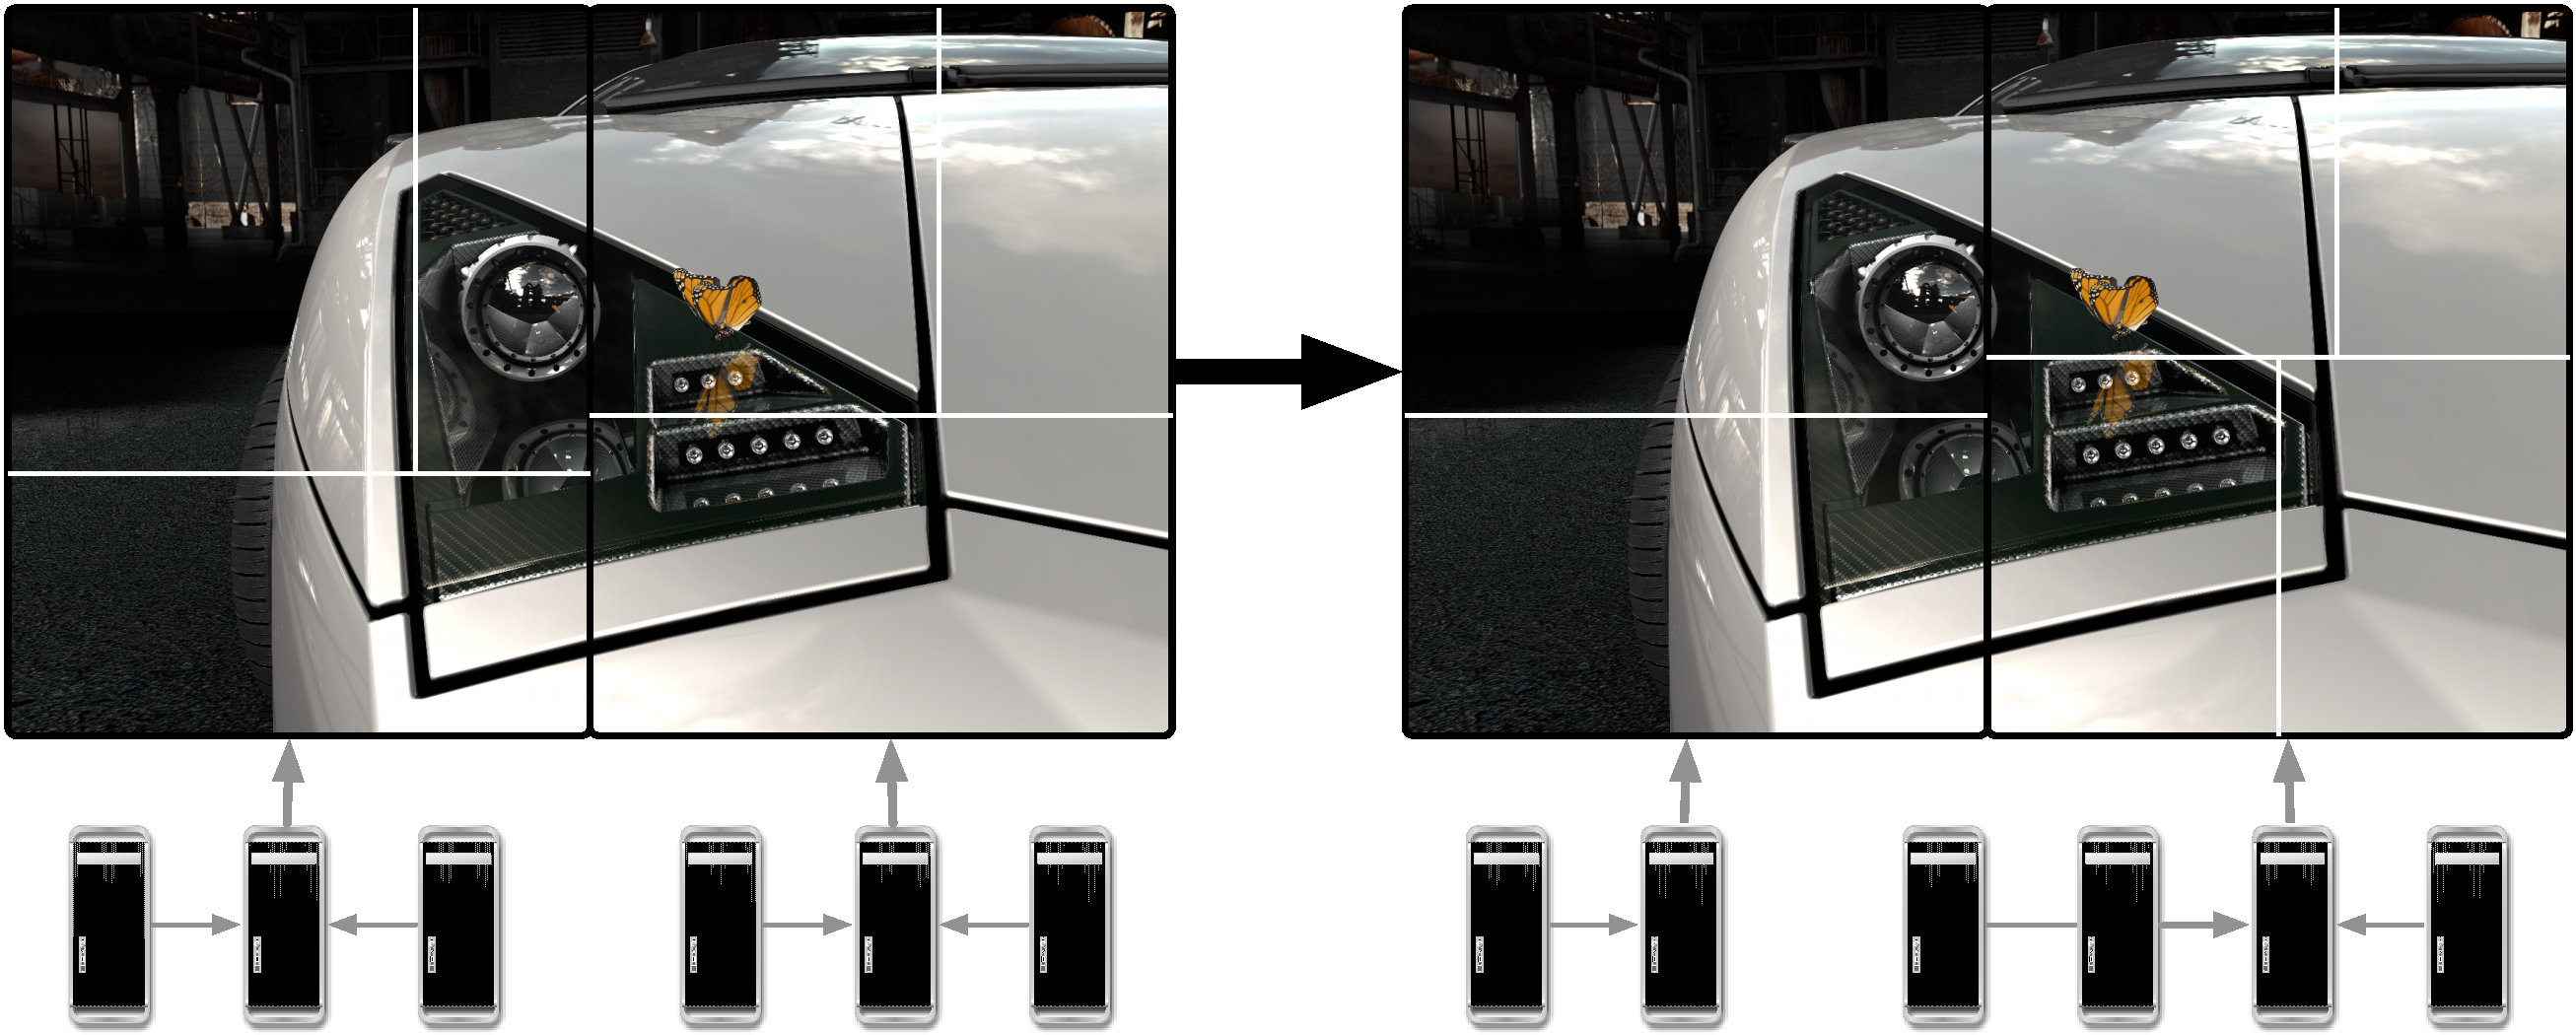
\includegraphics[width=.382\textwidth]{images/vieweq}
  \caption{\label{fvieweq}Cross-Segment Load-Balancing}
\end{wrapfigure}

The $m$ output channels typically each drive a display or projector of a
multi-display system. With CSLB, they are not required to be planar to each
other, that is, the algorithm works equally for tiled display wall and immersive
installations. Commonly, each destination channel is solely responsible for
rendering and/or compositing of its corresponding display segment.

A key element of CSLB is that the $m$ GPUs physically driving the $m$ display
segments will not be restricted in a one-to-one mapping to rendering tasks of
the corresponding display segment. In fact, CSLB performs dynamic assignment of
$n$ graphics resources from a pool to drive $m$ different destination display
segments, where the $m$ destination channel GPUs themselves may also be part of
the pool of graphics resources. Dynamic resource assignment is performed through
load-balancing components that exploit statistical data from previous frames for
the decision of optimal GPU usage for each segment as well as optimal
distribution of workload among them. The algorithm can easily be extended to use
predictive load-balancing based on a load estimation given the application.

CSLB is implemented in {\em Equalizer} as two layers of hierarchically organized
components, specified in the configuration. Figure~\ref{fViewEqualizer} depicts
a snapshot of a simple CSLB setup along with its configuration file. Two
destination channels, {\em Channel1} and {\em Channel2}, each connected to a
projector, create the final output for a multi-projector view. Each projector is
driven by a distinct GPU, constituting the source channels {\em Source1} and
{\em Source2}. But each source channel GPU can contribute to the rendering of
the other destination channel segment.

\begin{figure}[h!t] \center
  \subfigure[CSLB resources setup.]{\includegraphics[width=0.47\textwidth]{images/viewEqualizerSetup}
  \label{fViewEqualizerSetup}}
  \hfill
  \subfigure[CSLB configuration file format.]{
	\begin{minipage}[b]{0.46\textwidth}
	\setbox0=\vbox to 290pt{\tt\scriptsize
compound \\
\{ \\
\quad view\_equalizer \{\} \\
\quad compound \\
\quad \{ \\
\quad \quad channel "Channel1" \\
\quad \quad load\_equalizer\{\} \\
\quad \quad compound \{\} \# self \\
\quad \quad compound \\
\quad \quad \{ \\
\quad \quad \quad channel "Source2" \\
\quad \quad \quad outputframe \{\} \\
\quad \quad \} \\
\quad \quad inputframe\{\} \\
\quad \quad ... \\
\quad \} \\
\quad compound \\
\quad \{ \\
\quad \quad channel "Channel2" \\
\quad \quad load\_equalizer\{\} \\
\quad \quad compound \{\} \# self \\
\quad \quad compound \\
\quad \quad \{  \\
\quad \quad \quad channel "Source1"  \\
\quad \quad \quad outputframe \{\}  \\
\quad \quad \} \\
\quad \quad inputframe\{\} \\
\quad \} \\
\quad ... \\
\} \\
	\label{fViewEqualizerConfig}}
	\fbox{\box0}
	\end{minipage}
   }
\caption{A dual-GPU, dual-display cross-segment load-balancing setup: For each destination channel, a set of potential resources are allocated. A top-level {\em view\_equalizer} assigns the usage of each resource, based on which a per-segment {\em load\_equalizer} computes the 2D split to balance the assigned resources within the display. The left segment of the display has a higher workload, so, both {\em Source1} and {\em Source2} are used to render for {\em Channel1}, whereas {\em Channel2} makes use of only {\em Source2} to assemble the image for the right segment.}
\label{fViewEqualizer}
\end{figure}

CSLB uses a two-stage approach: a {\sf view\_equalizer} is attached to the top
level of the parallel rendering task decomposition compound hierarchy, and
handles the resource assignment. Each child of this root compound has one
destination channel, constituting one of the $m$ display segments, with a {\sf
load\_equalizer} or \textsf{tree\_equalizer} each. Hence the {\sf
view\_equalizer} supervises the different destination channels of a
multi-display setup. The {\sf load\_equalizer} on the other hand is
responsible for the partitioning of the rendering task among its child
compounds. Therefore, each destination channel of a display segment has its
source channel leaf nodes sharing the actual rendering load. One physical
graphics resource (GPU), being assigned to a source channel, can be referenced
in multiple leaf nodes and thus contribute to different displays. For
performance reason, one resource is at most assigned two rendering tasks, e.g.,
to update itself and to contribute to another display.

The rendered data, viewing configuration and user interaction will at runtime
produce different rendering loads for each segment of a multi-display system. As
the slowest segment will determine the overall performance of the system, it is
important to dynamically adjust load among segments. The {\sf view\_equalizer}
analyzes the load of all segments based on past frame rendering statistics and
adapts resource usage for each segment. For each rendered frame, the {\sf
view\_equalizer} sets the usage of each leaf source channel compound, to
activate or deactivate it for rendering on the given destination channel. This
usage setting is picked up by the per-segment load balancers, which will only
assign work proportionally to the usage, with no rendering task for $0$ usage.
\cite{EEP:11} provides a detailed description of the algorithm.

Cross-segment load balancing thus allows for optimal resource usage of multiple
GPUs used for driving the display segments themselves, as well as any additional
source GPUs for rendering. It combines multi-display parallel rendering with
scalable rendering for optimal performance. \cite{EEP:11} provides experimental
results for a six-monitor tiled display wall with up to 12 source GPUs, where
CSLB can more then double the framerate over a static resource assignment. A
strength of this algorithm lies in its flexibility. On one hand, it can perform
dynamic resource assignment not only for a planar display system as some
approaches which built a single virtual framebuffer for all output displays, but
also for curved displays and CAVE installations. On the other hand, it allows a
flexible assignment of potential contributing GPUs to each output channel
individually, that is, each output may have a different, potentially
overlapping, set of GPUs which may contribute to its rendering. \cite{EEP:11}
shows in its experiments that there is a sweet spot of the number of resources
per channel.

\section{Dynamic Frame Resolution}

The DFR equalizer (\fig{fdfr}) provides a functionality similar to dynamic
video resizing \cite{MBDM:97}, that is, it maintains a constant framerate by
adapting the rendering resolution of a fill-limited application. While the aforementioned uses a now-obsolete hardware implementation, our implementation is purely in software.

\begin{wrapfigure}{r}{.382\textwidth}
  \includegraphics[width=.382\textwidth]{images/dfr}
  \caption{\label{fdfr}Dynamic Frame Resolution}
\end{wrapfigure}
Dynamic frame resolution (DFR) works by rendering into a source channel
(typically on a FBO) separate to the destination channel, and then scaling the
rendering during the transfer (typically through an on-GPU texture) to the
destination channel. The DFR equalizer monitors the rendering performance and
accordingly adapts the resolution of the source channel and the zoom factor for
the source to destination transfer. If the performance and source channel
resolutions allow, this will not only subsample, but also supersample the
destination channel to reduce aliasing artefacts.

As with all other features, it can be combined with other scalability features,
e.g., sort-first rendering. It is also notable that it does not need any
additional code in the core compound logic, it simply exploits existing
functionality such as texture-based compositing frames and frame zoom with
dynamic per-frame adjustments.

\section{Frame Rate Equalizer}\label{sFramerateEq}

The framerate equalizer smoothens the output frame rate of a destination channel
by instructing the corresponding window to delay its buffer swap to a minimum
time between swaps. This is regularly used for time-multiplexed decompositions,
where source channels tend to drift and finish their rendering unevenly
distributed over time. This equalizer is however fully independent of DPlex
compounds, and may be used to smoothen irregular application rendering
algorithms. Due to the artificial sleep time before swap, it may incur a small
performance penalty, but it greatly improves the perceived rendering quality for
users in DPlex compounds.

\section{Monitoring}
\begin{wrapfigure}{r}{.382\textwidth}
  \includegraphics[width=.382\textwidth]{images/monitoreq}
  \caption{\label{fmonitor}Monitoring}
\end{wrapfigure}
The monitor equalizer (\fig{fmonitor}, \fig{fLayout}) allows to reuse the
rendering on another channel, typically for monitoring a larger setup on a
control workstation. Output frames on the display channels are connected to
input frames on a single monitoring channel. The monitor equalizer changes the
scaling factor and offset between the output and input, so that the monitor
channel has the same, but typically downscaled view, as the originating
segments. While this is not strictly a scalable rendering feature, it optimizes
resource usage by not needlessly rendering the same view multiple times.


\chapter{Data Distribution and Synchronization}


Most research in parallel rendering ignores the problem of managing applications
state in a distributed rendering setup. For research core scalability algorithms
this problem is trivially to solve, whereas in real-world applications it often
is one of the major challenges for using a distributed rendering cluster.

For this reason, we have spend a significant effort in researching, designing
and implementing a distributed execution layer which is used by Equalizer and
applications built on Equalizer. This {\em Collage} network library is an
independent open source project. In the following sections we highlight core
features and show how they are different from other distribution mechanisms,
e.g., the MPI library.

\section{Requirements}

The Collage network library was conceived with the requirements of a dynamic
parallel rendering system in mind. Some of the features implemented by Collage
came about later, and are often layered on top of the basic primitives. The core
requirements were:

\begin{compactdesc}

\item[Peer-to-peer network:] While the execution model of an Equalizer
application follows a master-slave approach, and Equalizer internally uses a
client-server model, the core transport layer should be agnostic to these
higher-level abstractions. In Collage, each communicating process is equal to
all others, and no traffic prioritization or communication pattern is enforced
by a node type. This has proven particularly useful during the implementation of
parallel compositing algorithms, where the compositing nodes form an ad-hoc
peer-to-peer network.

\item[Dynamic connection management:] As a consequence of the peer-to-peer
network, all nodes in a cluster are equivalent. Due to the heterogenous nature
of a parallel rendering application we felt the need to furthermore have no
constraints on the management of connections between nodes. Nodes are identified
and addressed by an universally unique identifier. The network layer lazily
establishes a connection to any given node, by querying its known neighbors or a
zeroconf network for connection parameters. Connections may be established
concurrently by both sides of a node pair (e.g. during parallel compositing),
which required the implementation of a robust handshake protocol during
connection establishment. For larger cluster installations, a fully connected
peer-to-peer network would be suboptimal, for example on Windows operating
systems there is a latency penalty once more than 64 connections are needed due
to some low-level implementation details.

\item[Transport layer abstraction:] The actual network protocol is abstracted
internally by an API requiring byte-oriented stream semantics. While this choice
of abstraction makes it harder for RDMA-based protocols to deliver full
performance, it has proven useful in supporting a large set of transports, from
standard Ethernet sockets, SDP for InfiniBand, native Verbs for Infiniband, UDT
to even a fully-featured multicast-over-UDP implementation. In particular the
ease of integration for multicast transport is strong evidence for the
usefulness of this abstraction.

\item[Convenient to use for existing applications:] The history and code
structure of visualization applications is often very different from distributed
applications such as simulation codes. They have been developed for years for
desktop systems, often are single-threaded and have data models and object
hierarchies built for their domain-specific problems and algorithms. The network
library needs to provide primitives which match this reality as closely as
possible by providing a modern, object-oriented C++ API for data distribution.

\end{compactdesc}


\section{Architecture}

Our Collage network library provides a peer-to-peer communication
infrastructure, offering different abstraction layers which gradually provide
higher level functionality to the programmer. Collage is used by Equalizer to
communicate between the application node, the server and the render clients.
\fig{fCollageUML} provides an overview of the major Collage classes and their
relationship. The main classes, in ascending abstraction level, are:

\begin{compactdesc}

\item[Connection:] A stream-oriented point-to-point communication line. Different
implementations of a connection exists. The connections transmit a raw byte
stream reliably between two endpoints for unicast connections, and between a set
of endpoints for multicast connections.

\item[DataOStream:] Abstracts the output of C++ data types onto a set of
  connections by implementing output stream operators. Uses buffering to
  aggregate data for network transmission.
\item[OCommand:] Extends DataOStream to implement the protocol between Collage
  nodes by adding node and command type routing information to the stream.
\item[DataIStream:] Decodes a buffer of received data into C++ objects and PODs
  by implementing input stream operators. Performs endian swapping if the
  endianness differs between the originating and local node.
\item[ICommand:] The other side of OCommand, extending DataIStream.
\item[Node and LocalNode:] The abstraction of a process in the cluster. Nodes
  communicate with each other using connections. A LocalNode listens on various
  connections and processes requests for a given process. Received data is
  wrapped in ICommands and dispatched to command handler methods. A Node is a
  proxy for communicating with a remote LocalNode.
\item[Object:] Provides object-oriented, versioned data distribution of C++
  objects between nodes within a session. Objects are registered or mapped on a
  Local\-Node.
\end{compactdesc}

\begin{figure}[h!t]\center
  \includegraphics[width=\textwidth]{images/collageUML}
  {\caption{\label{fCollageUML}UML class diagram of the major Collage classes}}
\end{figure}

\subsection{Connection}

A connection is the basic primitive used for communication between processes in
Collage. It provides a stream-oriented communication between two endpoints. A
connection is either closed, connected or listening. A closed connection cannot
be used for communications. A connected connection can be used to read or write
data to the communication peer. A listening connection can accept connection
requests.

A \textsf{ConnectionSet} is used to manage multiple connections. The typical use
case is to have one or more listening connections for the local process, and a
number of connected connections for communicating with other processes.
The connection set is used to select one connection which requires some action.
This can be a connection request on a listening connection, pending data on a
connected connection or the notification of a disconnect.

The connection and connection set can be used by applications to implement other
network-related functionality, e.g., to communicate with a sound server on a
different machine. A \textsf{LocalNode} has a connection set and uses this to
manage connections with other nodes.


\subsection{Command Handling}

Nodes and objects communicate using commands derived from data streams. The
basic command dispatch is implemented in the \textsf{Dispatcher} class, from
which \textsf{Node} and \textsf{Object} are sub-classed.

The dispatcher allows the registration of a commands with a dispatch queue and
an invocation method. Each command has a type and command identifier, which is
used to identify the receiver, registered queue and method. The dispatch pushes
the packet to the registered queue. When the commands are dequeued by the
processing thread the registered command method is invoked.

This dispatch and invocation functionality is used within Equalizer to dispatch
commands from the receiver thread to the appropriate node or pipe thread, and
then to invoke the command when it is processed by these threads. This
dispatching provides object-oriented semantics, since C++ instances can register
themselves on the dispatcher, and get automatically invoked in the correct
thread when an appropriate command arrives.

\subsection{Nodes}

The \textsf{Node} is the abstraction of one process in the peer-to-peer network.
Each node has a universally unique identifier. This identifier is used to
address nodes, e.g., to query connection information to connect to the node.
Nodes use connections to communicate with each other by sending
\textsf{OCommand}s.

The \textsf{LocalNode} is the specialization of the node for the given process.
It encapsulates the communication logic for connecting remote nodes, as well as
object registration and mapping. Local nodes are set up in the listening state
during initialization.

A remote \textsf{Node} can either be connected explicitly by the application or
due to a connection from a remote node. The explicit connection can be done by
programmatically creating a node, adding the necessary
\textsf{ConnectionDescription}s and connecting it to the local node. It may also
be done by connecting the remote node to the local node by using its
\textsf{NodeID}. This will cause Collage to query connection information for
this node from the already-connected nodes and zeroconf, instantiating the node
and connecting it. Both operations may fail.

\subsubsection{\label{sZeroconf}Zeroconf Discovery}

Each \textsf{LocalNode} provides a \textsf{Zeroconf} communicator, which allows
node and resource discovery. The service "\_collage.\_tcp" is used to announce
the presence of a listening \textsf{LocalNode} using the ZeroConf protocol to
the network. The node identifier and all listening connection descriptions are
announced, which is used to connect unknown nodes by using the node identifier
alone.

\subsubsection{Communication between Nodes}

\fig{fNetNode} shows the communication between two nodes. Each
\textsf{LocalNode} has a receiver thread, which uses a connection set to read
and dispatch incoming data from the network, and a command thread used for
higher-level functions such as object mapping. When the remote node sends a
command, the listening node receives the command and dispatches it from the
receiver thread. The dispatch will either invoke the bound function immediately,
or enqueue the command into the given queue. The queue consumer, for example the
main or command thread, will read the command of this queue and then invoke the
bound function.

\begin{figure}[h!t]\center
  \includegraphics[width=\textwidth]{images/netNode.pdf}
  {\caption{\label{fNetNode}Communication between two Nodes}}
\end{figure}


\section{Distributed, Versioned Objects}

Adapting an existing application for parallel rendering requires the
synchronization of application data across the processes in the parallel
rendering setup. Existing parallel rendering frameworks address this often
poorly, at best they rely on MPI to distribute data. Real-world, interactive
visualization applications are typically written in C++ and have complex data
models and class hierarchies to represent their application state. As outlined
in \cite{EMP:09}, the parallel rendering code in an \textsf{Equalizer}
application only needs access to the data needed for rendering, as all
application logic is centralized in the application main thread. We have
encountered two main approaches to address this distribution: Using a shared
filesystem for static data, or using data distribution for static and dynamic
data. Distributed objects are not required to build \textsf{Equalizer}
applications. While most developers choose to use this abstraction for
convenience, we have seen applications using other means for data distribution,
e.g., MPI.

Distributed objects in \textsf{Collage} provide powerful, object-oriented data
distribution for C++ objects. They facilitate the implementation of data
distribution in a cluster environment. Distributed objects are created by
subclassing from \textsf{co::Serializable} or \textsf{co::Object}. The
application programmer implements serialization and deserialization. Distributed
objects can be static (immutable) or dynamic. Objects have a universally unique
identifier (UUID) as cluster-wide address. A master-slave model is used to
establish mapping and data synchronization across processes. Typically, the
application main loop registers a master instance and communicates the UUID to
the render clients, which map their instance to the given identifier. The
following object types are available:

\begin{compactdesc}
\item[Static] The object is not versioned nor buffered. The instance data is
  serialized whenever a new slave instance is mapped. No additional data is
  stored.
\item[Instance] The object is versioned and buffered. The instance and delta
  data are identical; that is, only instance data is serialized. Previous
  instance data is saved to be able to map old versions.
\item[Delta] The object is versioned and buffered. The delta data is typically
  smaller than the instance data. The delta data is transmitted to slave
  instances for synchronization. Previous instance and delta data is saved to be
  able to map and sync old versions.
\item[Unbuffered] The object is versioned and unbuffered. No data is stored, and
  no previous versions can be mapped.
\end{compactdesc}

Serialization is facilitated using output or input streams, which abstract the
data transmission and are used like a \textsf{std::stream}. The data streams
implement efficient buffering and compression, and automatically select the best
connection for data transport. Custom data type serializers can be implemented
by providing the appropriate serialization functions. No pointers should be
directly transmitted through the data streams. For pointers, the corresponding
object is typically a distributed object as well, and its UUID and version are
transmitted in place of a pointer.

Dynamic objects are versioned, and on \textsf{commit} the delta data from the
previous version is sent, if available using multicast, to all mapped slave
instances. The data is queued on the remote node, and is applied when the
application calls \textsf{sync} to synchronize the object to a new version. The
\textsf{sync} method might block if a version has not yet been committed or is
still in transmission. All versioned objects have the following characteristics:

\begin{compactitem}
\item The master instance of the object generates new versions for all
  slaves. These versions are continuous. It is possible to commit on slave
  instances, but special care has to be taken to handle possible
  conflicts.
\item Slave instance versions can only be advanced; that is, \textsf{sync(
  version)} with a version smaller than the current version will fail.
\item Newly mapped slave instances are mapped to the oldest available
  version by default, or to the version specified when calling
  \textsf{mapObject}.
\end{compactitem}

\label{sec:Serializable}The \textsf{Collage} Serializable implements one
convenient usage pattern for object data distribution. The
\textsf{co::Serializable} data distribution is based on the concept of dirty
bits, allowing inheritance with data distribution. Dirty bits form a 64-bit mask
which marks the parts of the object to be distributed during the next commit.
For serialization, the application developer implements \textsf{serialize} or
\textsf{deserialize}, which are called with the bit mask specifying which data
has to be transmitted or received. During a commit or sync, the current dirty
bits are given, whereas during object mapping all dirty bits are passed to the
serialization methods.

Blocking commits allow to limit the number of outstanding, queued versions on
the slave nodes. A token-based protocol will block the commit on the master
instance if too many unsynchronized versions exist.

\subsubsection{Optimizations}

The API presented in the previous section provides sufficient abstraction to
implement various optimizations for faster mapping and synchronization of data:
compression, chunking, caching, preloading and multicast.

The most obvious one is compression. Recently, many new compression algorithms
have been developed which exploit modern CPU architectures and deliver
compression rates well above one gigabyte per second. \textsf{Collage} uses the
Pression library~\cite{pression}, which provides a unified interface for a
number of compression libraries, such as FastLZ~\cite{jesperfast},
Snappy~\cite{snappy} and ZStandard~\cite{zstd}. It also contains a custom,
virtually zero-cost RLE compressor. Pression parallelizes the compression and
decompression using data decomposition. This compression is generic and
lossless, implemented transparently for the application. Applications can also
use data-specific compression.

The data streaming interface implements chunking, which pipelines the
serialization code with the network transmission. After a configurable number of
bytes has been serialized to the internal buffer, it is transmitted and
serialization continues. This is used both for the initial mapping data and for
commit data.

Caching retains instance data of objects in a client-side cache, and reuses this
data to accelerate mapping of objects. The instance cache is either filled by
``snooping'' on multicast transmissions or by an explicit preloading when the
master objects are registered. The preloading sends instance data of recently
registered master objects to all connected nodes, while the corresponding node
is idle. These nodes simply enter the received data to their cache. Preloading
uses multicast when available.

Due to the master-slave model of data distribution, multicast is used to
optimize the transmission time of data. If the contributing nodes share a
multicast session, and more than one slave instance is mapped, \textsf{Collage}
automatically uses the multicast connection to send the new version information.

In \cite{ESP:18} we provide an extensive analysis of data compression, buffering
and multicast in practical scenarios, and show that they can provide substantial
speedups for data distribution.

%------------------------------------------------------------------------------
\subsection{Reliable Stream Protocol}\label{sec:RSP}

RSP is an implementation of a reliable multicast protocol over unreliable UDP
multicast transport. RSP behaves similarly to TCP; in contrast to the underlying
UDP transport, it is not message-oriented but implements byte stream semantics.
RSP provides full reliability and ordering of the data, and slow receivers will
eventually throttle the sender through a sliding window algorithm. This behavior
is needed to guarantee delivery of data in all situations. Pragmatic generic
multicast (PGM~\cite{pgm}) provides full ordering, but slow clients will
disconnect from the multicast session instead of throttling the send rate. Since
we use multicast for distributing application data to all rendering clients we
want semantics similar to TCP, that is, waiting for a client to read data is
preferable over loosing this client.

RSP combines various established multicast
algorithms~\cite{adamson2004negative,Gau:2002} in an open source implementation
capable of delivering wire speed transmission rates on high-speed LAN
interfaces. In the following we will outline the RSP protocol and implementation
as well as motivate the design decisions. Any defaults given below are for Linux
or OS X, the Windows UDP stack requires different default values which can be
found in the implementation.

Our RSP implementation uses a separate protocol thread for each RSP group, which
handles all reads and writes on the multicast UDP socket. It implements the
protocol handling and communicates with the application threads through
thread-safe queues. The queues contain datagrams filled with the application
byte stream, prefixed by a header of at most eight bytes. Each connection has a
configurable number of buffers (1024 by default) of a configurable MTU (1470
bytes default), which are either free or in transmission. The header contains
two bytes for the datagram type (connection handshake, data, acknowledgment,
negative acknowledgment, acknowledgment request), and up two six bytes of
datagram-specific information (e.g. for acknowledgment: two bytes read node
identifier, two bytes write node identifier, two bytes sequence number).

\fig{fRSP} shows the data flow through the RSP implementation. Each member of the multicast group opens a listening connection, which will send query datagrams to the multicast socket. For each found member, a receiving connection instance is created and, similar to a TCP socket, passed to the application upon \textsf{accept}. Each connection instance has a fixed number (1024 by default) of fixed-size (1470 by default) buffers, each used directly as an UDP datagram. The listening connection uses these buffers for writing data, and each receiving connection uses its buffers for received data. These buffers are continuously cycled through two sets of queues: a blocking, thread-safe queue used on the application side for reading and writing data, and a non-blocking, lock-free and thread-safe queue on the protocol thread for data management.

\begin{figure}[h!t]\center
  \includegraphics[width=\textwidth]{images/rspPackets.pdf}
  {\caption{\label{fRSP}RSP data flow}}
\end{figure}

When writing data, the application thread pops empty buffers from its queue
(blocking when the data cannot be written fast enough), fills in the
\textsf{data} datagram headerm and copies the application data piece-wise into
the datagram. The datagrams are then pushed onto the protocol thread buffer
queue. The protocol thread writes the datagrams unto the UDP multicast socket,
and reads and handles any incoming datagrams. On the receiver side, the protocol
receives the data, and pushes them in order to the corresponding application
thread queue. Out-of-order datagrams are stored aside and queued in order later,
and a negative acknowledgments (nack) are immediately sent for missing
datagrams. The writer will repeat nack'd datagrams, recycle fully acknowledged
datagrams to the application queue, and ask for missing acknowledgments if
needed. When reading data, the application pops full buffers from the
corresponding connection's queue (blocking when no data is available), copies
the data piece-wise out of datagram into the application buffer, and recycles
the cleared buffers onto the protocol thread queue.

Handling a smooth packet flow is critical for performance. RSP uses active flow
control to advance the byte stream buffered by the implementation. Each incoming
connection actively acknowledges every $n$ (17 by default) packets fully
received. The incoming connections offset this acknowledgment by their
connection identifier to avoid bursts of acks. Any missed datagram is actively
nack'ed as soon as detected. Write connections continuously retransmit packets
for nack datagrams, and advance their window upon reception of all acks from the
group. The writer will explicitly request an ack or nack when it runs out of
empty buffers or finishes its write queue. Nack datagrams may contain multiple
ranges of missed datagrams, which is motivated by the observation that UDP
implementations often drop multiple contiguous packets.

Congestion control is necessary to optimize bandwidth usage. While TCP uses the
well-known additive increase, multiplicative decrease algorithm, we have chosen
a more aggressive congestion control algorithm of additive increase and additive
decrease. This has proven experimentally to be more optimal: UDP is often
rate-limited by switches; that is, packets are discarded regularly and not
exceptionally. Only slowly backing of the current send rate helps to stay close
to this limit. Furthermore, our RSP traffic is limited to the local subnet,
making cooperation between multiple data stream less of an issue. Send rate
limiting uses a bucket algorithm, where over time the bucket fills with send
credits, from which sends are substracted. If there are no available credits,
the sender sleeps until sufficient credits are available.

In \cite{ESP:18} we provide experimental results, showing that our
implementation can achieve above 90\% wire speed on 10~GBit/s Ethernet, shows
good scalability with respect to the multicast group size, and is very effective
for distributing structured and unstructured application data to a large number
of rendering clients concurrently.

\chapter{Conclusion}

\section{Future Work}


\if 0

 \chapter{Problem Statement}

 Visualization of large amounts of data has been always been encumbered by
 sufficient system software. Compared to other domains, such as HPC simulations,
 large data visualization has received relatively little attention in both
 research and development. Consequently, there is a large amount of data which
 has not been explored sufficiently. In particular in scientific visualization,
 where data is often spatial and temporal, even simple visualizations can extract
 new information and provide a valuable tool to domain scientists for discovery.

 The central theme of the proposed research is therefore: {\bf How can we improve
 the capabilities of existing visualization algorithms for rendering large
 amounts of data?} This generic problem can be researched more concretely along
 the following research questions:
 \begin{compactenum}
  \item How can we improve the rendering performance of visualization applications to enable users to explore more data?
  \begin{compactenum}
   \item What new algorithms will decrease the time needed to composite rendering results, in particular for sort-last rendering?
   \item How can we improve load-balancing for sort-first rendering, in particular for large display systems?
  \end{compactenum}
  \item How can we reduce end-to-end system latency for better user experience?
  \begin{compactenum}
   \item In a generic parallel rendering framework, how can we schedule the different rendering stages to minimize the latency for the user?
   \item How can we architect the parallel rendering framework to minimize synchronization between threads?
  \end{compactenum}
  \item How can we maximize the impact of this research on large data scientists?
 \end{compactenum}

 The obvious solution to the problem is to utilize more compute resources to
 parallelize and scale the rendering algorithm. The goal can either be to
 increase strong scaling (render a given data set faster) or weak scaling (render
 a larger data set at roughly the same speed). To efficiently use more resources,
 we need to research increasing the parallelism of existing algorithms, and to
 reduce the bottleneck in the image compositing stage.

 An important collateral problem is the overall latency of the rendering system,
 that is, the time between a user input and its resulting output frame. While
 this is lower-bounded by the framerate of the rendering, oftentimes algorithmic
 or implementation choices increase the total system latency. Often this is a
 side effect of improving the rendering performance, but it also decreases the
 usability of the application for interactive usage. One typical example is
 pipelining of operations in the rendering pipeline.

 Visualizing large amounts of data often goes hand in hand with the usage of
 high-resolution displays. Since large amounts of data tends to have a lot of
 detail, high-resolution desktop screens (4K or 8K resolution), as well as
 high-resolution display walls, help tremenduously in recognising and
 understanding details of the data. The high resolution however aggravetes all
 the aforementioned problems: The increased pixel count reduces rendering
 performance, requires better compositing algorithms, and increases the latency
 due to longer transfer times during compositing and display. Since pixel count
 increases quadratically with display size, this problem will become more
 important as display resolution increases.

 \chapter{Proposed Solution} % 2-6

 Parallel rendering has received a lot of attention in the last couple of
 decades, yet libraries and frameworks to develop parallel rendering applications
 are scarcely available. Consequently, there are only a few applications which
 can utilize parallelism for rendering, let alone do so efficiently at scale.
 This research proposes to address these shortcomings by developing {\bf reusable
   software components} to make parallel rendering programs easier to develop, by
 generalizing existing research into reusable software implementations.

 Based on these foundations, we propose to research new algorithms to improve
 rendering performance. In particular we see potential in improving the
 scalability through better {\bf load balancing}, {\bf image compositing}
 algorithms, and {\bf holistic optimization} of the whole rendering pipeline
 under control of our framework. Orthogonally to this algorithmic research, we
 propose to research {\bf data processing and data access} strategies for
 parallel rendering applications. This is particularly important, yet
 underdeveloped, in the context of the visual analysis for HPC simulation
 results.

 Previous parallel rendering approaches typically failed in one of the following
 system requirements:
 %
 \begin{compactenum}
  \item generic application support, instead of domain-specific solution
  \item scalable abstraction of the graphics layer
  \item exploit existing code infrastructure, such as proprietary scene graphs, molecular data structures, level-of-detail and geometry databases
 \end{compactenum}

 To date, generic and scalable parallel rendering frameworks that can be adopted
 to a wide range of scientific visualization domains are not yet readily
 available. Furthermore, flexible configurability to arbitrary cluster and
 multi-display configurations has also not been addressed in the past, but is of
 immense practical importance to scientists depending on high-performance
 interactive visualization as a scientific tool. We propose a novel flexible
 framework for parallel rendering that supports scalable performance,
 configuration flexibility, is minimally invasive with respect to adapting
 existing visualization applications, and is applicable to virtually any
 scientific visualization application domain.

 To that end, this work aims to significantly advance the system design and
 implementation of flexible, distributed and cluster-parallel rendering
 frameworks as well as algorithms and system design for large data processing in
 the context of interactive visualization. The core of this proposal is the
 Equalizer project, a foundation for scalable, multi-GPU visualization software
 in all application domains. The main contributions of such a parallel rendering
 system are:
 %
 \begin{compactenum}
  \item novel concept for flexible runtime configuration of graphics system resources
  \item easy specification of parallel task decomposition and image compositing algorithms
  \item automatic decomposition and distributed execution of rendering tasks according to the configuration
  \item support for polygonal and volume rendering for opaque and transparent geometries
  \item fully decentralized software architecture providing network swap barrier synchronization and data distribution functionality
  \item support for low-latency distributed frame synchronization and image compositing
  \item minimally invasive programming model
 \end{compactenum}

 The broader impact of this work revolves around the development and improvement
 of a generic, flexible and scalable parallel rendering infrastructure applicable
 to a large number of application domains. The expected improvements of the
 proposed activities in distributed parallel parallel rendering will be
 integrated into open source software libraries and as such will be available to
 the general public and especially to developers of high-performance
 visualization and interactive rendering applications. This approach will
 maximize the impact of this research on large data scientists (research question
 4).

 A strong focus during the development is to architect the framework for
 scalability to address research questions 1 and 2. Based on my previous work and
 the study of existing implementations, scalability in parallel rendering today
 is mostly limited by excessive synchronization between execution threads,
 imbalance in the task decomposition, and compositing performance. Equalizer only
 has the following necessary synchronization points:
 %
 \begin{compactenum}
  \item Swap synchronization between output channels to the same display system
  \item Finalization of rendering frames given a configurable latency for all render threads
  \item Availability of image data for compositing between the source and destination threads
 \end{compactenum}
 %
 This architecture has proven to provide good scalability by inherently allowing
 the pipelining of data synchronization, rendering and compositing tasks
 (research question 1), while simultaneously minimizing the time to display
 results by letting render threads execute as early as possible (research
 question 2). Furthermore, this will provide better scalability for the more
 specific research questions 1(a) and 1(b).

 The following publications are planned or already published to address the corresponding research question:
 \begin{compactenum}
  \item
  \begin{compactenum}
   \item In \cite{EP:07, MEP:10, EBAHMP:12} we presented different algorithms to optimize the compositing step for sort-last rendering and optimisations for modern multi-GPU NUMA nodes.
   \item In \cite{EEP:11, SPEP:16} we presented novel load-balancing algorithms for sort-first rendering.
  \end{compactenum}
  \item Our first system paper \cite{EMP:09} introduces the architecture of a parallel rendering framework with minimal synchronization and optimized task scheduling, including an in-depth experimental analysis. \cite{EBAHMP:12} introduced further scheduling optimizations.
  \item Our foundation systems paper \cite{EMP:09} and applications work \cite{HBBES:13} provide evidence on the sustainability of our approach. We submitted a follow-on systems paper to ACM Transactions on Visualization and Graphics \cite{ESP:18}. This paper also contains background on applications and integrations of Equalizer in other software packages.
 \end{compactenum}

 Based on this generic parallel rendering framework, we propose to research
 concrete algorithms and applications. We propose an engineering-driven approach
 which will analyse existing algorithms, improve them incrementally by focusing
 on one aspect of a large data application, and then compare our new research
 against existing work. Since our research questions are largely performance
 related, this comparison will be in most cases performed through benchmarking.
 In particular, we see potential in:
 %
 \begin{compactdesc}
  \item [Load-balancing for rendering resources:] While basic algorithms have been
  proposed for reactive and proactive load-balancing of simple rendering tasks,
  research is still needed for improving the resource utilisation for large-scale
  parallelization, as well as for rendering in more complex multi-display
  environments such as tiled display walls and immersive installations. The
  results of this research is directly measurable through application benchmarking
  of representative data sets. We consider this research goal achieved if we
  proposed and implemented new algorithms which can consistently deliver better
  performance over existing work, addressing research question 1(b).
  \item [Compositing of the rendering results:] Previous research has focused on
  the scalability for very large scale HPC runs in the order of hundreds of
  thousands of cores, which are oftentimes not interactive by nature. We propose
  to improve image compositing performance for interactive applications on
  medium-sized (up to hundreds of GPUs) visualization clusters through analysing
  and optimising image compositing algorithms. As with load-balancing, this area
  of research can be considered achieved if benchmarks show consistent improvement
  over state of the art algorithms, addressing research question 1(a).
  \item [Applications for parallel rendering:] While a few parallel rendering
  applications exist, developing them is still a significant undertaking. We
  propose to extend existing rendering applications and algorithms for scientific
  visualization for parallel rendering. Not only will this create new results and
  capabilites for large data visualization, it also improves the general
  applicability and ease of use of our generic parallel rendering components. We
  consider this goal achieved if our framework is used in multiple visualization
  applications. A side effect of this goal is addressing research question 4.
  \item [Data management for visualization of HPC data:] We see a substantial
  potential in combining big data management strategies from the cloud computing
  domain to processing and visualising HPC simulation data. Paradoxically, storage
  systems for HPC are often optimised for large, sequential access, which is
  predominant during write, but not typical for analysis and visualization which
  use more, but smaller scattered read accesses. This is an exploratory research
  goal, where we hope to demonstrate the usefulness of cloud computing storage
  systems for HPC storage and linked large data visualizations. We consider this
  goal reached if we evaluated multiple approaches to data storage against their
  traditional parallel filesystem implementation, and can make recommendations for
  future research. The evaluation will again be benchmark-based, by measuring the
  time to solution for typical data access patterns.
 \end{compactdesc}

 This research will have a sustainable impact on how we use large-scale
 visualization systems as their commoditization makes them affordable to many
 more organizations. This is due to the research approach of using an
 incremental, engineering-driven and data-validated strategy, open source
 implementation of most software artefacts, the development of high-quality
 foundations, as well as the collaboration with both research and industry
 partners during the research.

 The proposed research will have a direct, significant impact on accelerating the
 simulation-based research performed in the Blue Brain Project. On one hand, the
 data distribution capabilities will allow faster development of scalable,
 neuroscience-specific visualization applications for the BBP. This is of
 particular importance as we foresee the need to visualize different modalities
 at different brain scales as the simulations grow in complexity and data size in
 the future.

 \chapter{Research Plan\label{sPlan}}

 The proposed research is heavily based on prior software engineering work in the
 domain, and will leverage a strong parallel rendering system to enable novel
 research within a non-trivial software stack. Consequently, a large portion of
 the plan is the development of the parallel rendering framework, where the
 timeline has been reverse-engineered from the work performed leading to this
 proposal.

 The integration of these frameworks into applications is not part of this
 research schedule, since it is a non-research activity. These developments have
 been and will be funded by other means. This work is nevertheless an important
 part of this project, as it validates the general applicability of this research
 in academia and industry.
 \clearpage
 The research is structured as follows:
 %
 \begin{compactdesc}
  \item[M1-3: System Architecture:] Outline the general system architecture,
  configuration structure and entities, class hierarchy and API. Research
  third-party technologies to be used in the implementation.
  \item[M4-10: Distributed Execution Layer:] First iteration of the implementation
  of the distributed execution layer allowing dynamic configurations and
  communication patterns.
  \item[M10-16: Multi-Display Parallel Rendering Framework:] Based on the
  distributed execution layer, develop a first parallel rendering framework
  capable of driving multi-display environments for monoscopic rendering,
  including the automatic launch of the rendering processes from the main
  application.
  \item[M17: Stereoscopic Rendering:] Implement stereoscopic rendering using
  configurable interocular distance.
  \item[M18: Immersive Rendering:] Head-tracking API and configuration entities,
  calculation of corresponding off-axis frusta.
  \item[M19: Scalable Rendering Architecture:] Design configuration and class
  hierarchy for scalable rendering modes, including task decomposition and
  parallel compositing algorithms.
  \item[M20-24: Basic Scalable Rendering:] Implement basic decompositions (2D, DB,
  Eye) and corresponding parallel compositing algorithms (2D, direct-send,
  binary-swap).
  \item[M25-30: Advanced Scalable Rendering:] Implement advanced compounds (Pixel,
  DPlex) and compositing optimizations (realtime image compression, region of
  interest, etc.).
  \item[M30-32: First Publication:] Benchmarking and systems paper.
  \item[M33-36: Load Balancing:] Implement load-balancing for multi-display
  setups. improved automatic load-balancing using region of interest.
  \item[M37-38: Second Publication:] Benchmarking and load-balancing paper.
  \item[M39-42: Compositing Research:] Research compositing optimizations.
  \item[M43-44: Third Publication:] Benchmarking and compositing paper.
  \item[PhD Proposal]
  \item[M45-46: Fourth Publication:] Benchmarking and updated systems paper.
  \item[M47-52: Dissertation:] Write and defend dissertation.
 \end{compactdesc}

\fi

%%%%%%%%%%%%%%%%%%%%%%%%%%%%%%%%%%%%%%%%%%%%%%%%%%%%%%%%%%%%%%%%%%%%%%%%%%%%%%%%
% Back matter for thesis
%%%%%%%%%%%%%%%%%%%%%%%%%%%%%%%%%%%%%%%%%%%%%%%%%%%%%%%%%%%%%%%%%%%%%%%%%%%%%%%%


%--------------------------------------------------------------------------------
% Appendix
%--------------------------------------------------------------------------------
%%%%%%%%%%%%%%%%%%%%%%%%%%%%%%%%%%%%%%%%%%%%%%%%%%%%%%%%%%%%%%%%%%%%%%%%%%%%%%%%
% Appendix style
%%%%%%%%%%%%%%%%%%%%%%%%%%%%%%%%%%%%%%%%%%%%%%%%%%%%%%%%%%%%%%%%%%%%%%%%%%%%%%%%


\definecolor{numColor}{rgb}{0.22,0.37,0.56}

% The first makeatletter is to define the chapter layout in the real "Chapter" chapters

\makeatletter
\def\@makechapterhead#1{%
%    \vspace*{10\p@}%
%    \hrule

    \line(1,0){0}
    \newline
    {
         %\begin{tabular}{|@{}l|r@{}@{}|}
	 \begin{tabular}{@{}lr@{}@{}} 
	 %\hline
	 \linethickness{ 4px }\color{numColor}\line(1,0){260} 
	 & \multirow{2}{*}{\fontsize{100}{62}\usefont{OT1}{ptm}{m}{n}\selectfont \color{numColor} \thechapter}\\ % ptm
	 & \\ 
	 % \Huge \bfseries \usefont{OT1}{phv}{m}{n}\selectfont \scshape\@chapapp \hspace{8.25cm} & \\
	 %\scshape \bfseries\Huge \@chapapp \hspace{8.25cm}
	 \scshape \LARGE \usefont{T1}{fvs}{sc}{n}\selectfont \letterspace to 2.5\naturalwidth{APPENDIX} \hspace{19mm}
	 & \\ 
	 %\hline
	 \end{tabular}

         \vskip 100\p@
         \raggedleft
         \interlinepenalty\@M
         \scshape \fontsize{24}{30} \usefont{T1}{fvs}{n}{n}\selectfont \scshape \MakeUppercase{#1}\par\nobreak
         \vskip 80\p@%60
    }
}


\appendix


%--------------------------------------------------------------------------------
% Bibliography
%--------------------------------------------------------------------------------
\bibliographystyle{apalike}
\bibliography{references/references}


%--------------------------------------------------------------------------------
% Curriculum Vitae
%--------------------------------------------------------------------------------
% LATEX BUG: chapter* following the bibliography show always the bibliography header. Workaround: change header manually
\markboth{CURRICULUM VITAE}{}
%%%%%%%%%%%%%%%%%%%%%%%%%%%%%%%%%%%%%%%%%%%%%%%%%%%%%%%%%%%%%%%%%%%%%%%%%%%%%%%%
% Curriculum Vitae
%%%%%%%%%%%%%%%%%%%%%%%%%%%%%%%%%%%%%%%%%%%%%%%%%%%%%%%%%%%%%%%%%%%%%%%%%%%%%%%%


%--------------------------------------------------------------------------------
% Header
%--------------------------------------------------------------------------------
\chapter*{Curriculum Vitae}
\addcontentsline{toc}{chapter}{Curriculum Vitae}


%--------------------------------------------------------------------------------
\section*{Personal Information}
%--------------------------------------------------------------------------------
\vspace{-5pt}
\begin{table}[h] %\centering
\begin{tabular}{@{} p{2.25cm} p{0.8\textwidth}}
Name            & Fatih Erol \\
Date of birth   & XXXXXX XX, 19XX \\
Place of birth  & Trabzon, Turkey
\end{tabular}
\end{table}
\vspace{-10pt}


%--------------------------------------------------------------------------------
\section*{Education}
%--------------------------------------------------------------------------------
\vspace{-5pt}


%--------------------------------------------------------------------------------
\section*{Publications}
%--------------------------------------------------------------------------------
\subsection*{Conference Publications}
\subsection*{Journal Articles}


\end{document}
%%%%%%%%%%%%%%%%%%%%%%%%%%%%%%%%%%%%%%%%%%%%%%%%%%%%%%%%%%%%%%%%%%%%%%%%%%%%%%%%
